\subsection{Classification by Decision Trees}
\label{section:method1}

%Die Feature Extraction findet in der Matlab Function GetFeatures.m statt. Hier wird ein Feature Vektor aus verschiedenen Eigenschaften eines Frames erstellt.
%Auch hier muss beachtet werden, dass die spätere Software in Realtime lauffähig sein soll. Deshalb muss eine Drum oder ein Becken nach dem Schlag möglichst schnell erkannt werden. Es können also nur Bereiche im Audiofile betrachtet werden, die sich unmittelbar nach dem Onset befinden. Außerdem soll der Feature Vektor aus möglichst wenigen Werten bestehen, um eine möglichst kurze Laufzeit bei der anschließenden Klassifizierung zu gewährleisten.
The first approach to the problem of classification was to extract a feature vector out of the recorded data and apply it to an existing classification algorithm. After the recorded audio data is pre-processed, the features are extracted by using MatLab\textsuperscript{\textregistered}. To be able to use the extracted features with Weka, they are written into a .csv file. In Weka, different classification algorithms are applied to the data. The best results are gained by the use of decision trees. Thus, decision trees are used to test different compositions of features.

\subsubsection{Pre-Processing}

\label{section:method1pre-processing}
Before the features can be extracted, the recorded data needs to be pre-processed. The pre-processing starts with the onset detection and the extraction of the subsequent window \lstinline{w}. This window \lstinline{w} contains the attack of the stroke. It further calculates three subsequent, overlapping frames \lstinline{w1}, \lstinline{w2} and \lstinline{w3} from the window \lstinline{w}. Subsequently, the four resulting windows are processed by Fourier transform, noise reduction and normalization. For the training data, the training method, which is explained in section \ref{section:training}, is applied.

For the detection of the onset the algorithm described in section \ref{section:onsetdetectionmethod} is used. Since every test and training recording includes only one stroke, the first found onset is declared as the starting point of the window \lstinline{w}. Based on the window size of the training data in section \ref{section:training}, the size of \lstinline{w} is set to 2048 samples. To receive the three frames, the window \lstinline{w} is split into three subsequent frames that are overlapping about halve their size. The size of the frames is half the size of the initial window \lstinline{w}. Thus, as shown in figure \ref{fig:frames}, if the initial window includes 2048 samples, the new windows have a size of 1024 samples and are overlapping by 512 samples.

\begin{figure}[htb]
	\centering
	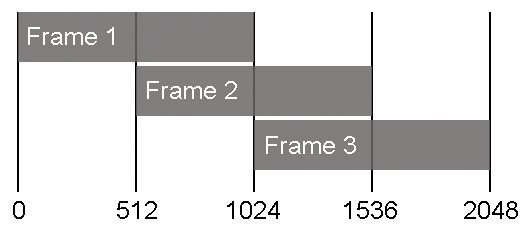
\includegraphics[height=3cm]{images/frames.png}
	\label{}
	\caption{Three subsequent frames with the size of 1024 samples, overlapping by 512 samples.}
	\label{fig:frames}
\end{figure}

After extracting window \lstinline{w} and the subsequent frames \lstinline{w1}, \lstinline{w2} and \lstinline{w3}, the containing audio information is transformed to their frequency spectra by applying MatLab\textsuperscript{\textregistered}s FFT function with a Hamming window. The resulting spectra are shortened to half their sizes because the values are repeated reversely from the middle of the spectrum. Thus, the duplicated values are removed.

Since the recorded data includes a low frequent noise from 0 Hz to 40 Hz, the first two frequency bins are set to zero. These bins include the frequency spectrum from 0 Hz to 43 Hz. Thus, the noise frequencies are removed from the spectrum. A more variable method for noise reduction is used for the second classification method, which is described in section \ref{section:method2}.

Finally, the normalization is performed to get comparable values for the amplitudes of different powered strokes. Therefore, every value in the windows \lstinline{w}, \lstinline{w1}, \lstinline{w2} and \lstinline{w3} is divided by the appropriate window's maximum. Hence, the maximum value in the resulting normalized arrays is one.

The pre-processing is done by a MatLab\textsuperscript{\textregistered} function called \lstinline{prepareTrainingData()}, which is used for the training records and a function called \lstinline{prepareTestData()}, which is used for the test records. The function receives the audio data as matrix \lstinline{testdata} and the window size as value \lstinline{windowSize}. It returns the windows \lstinline{w}, \lstinline{w1}, \lstinline{w2} and \lstinline{w3} for each data set as the matrices \lstinline{W}, \lstinline{W1}, \lstinline{W2} and \lstinline{W3}.

\subsubsection{Feature Extraction}
\label{section:method1Features}

The feature extraction is based on the pre-processed frequency spectrum of the drum strokes. As described in the preceding sections, a frequency band from 0 Hz to 22.050 Hz is considered in the four different windows \lstinline{w}, \lstinline{w1}, \lstinline{w2} and \lstinline{w3}. To reach a good calculation time for the feature extraction, the number of used features is a decisive factor. The less features there are needed to classify the drum type, the less calculation time is made demands on. The extracted features are saved as a .csv file which can be read by Weka. 

The MatLab\textsuperscript{\textregistered} implementation for the feature extraction is realized by the function \lstinline{getFeatures}. The function receives the Fourier transformed window from which it extracts 20 different features. Thereby, only half of the frequency spectrum is considered because the values are repeated reversely from the middle of the spectrum. The chosen features are single values saved in variables of the data type double. The following features are extracted:

\begin{itemize} 
	\item Maximum peak 1 amplitude and frequency (\lstinline{peak1A}, \lstinline{peak1F})
	\item Maximum peak 2 amplitude and frequency (\lstinline{peak2A}, \lstinline{peak2F})
	\item Maximum peak 3 amplitude and frequency (\lstinline{peak3A}, \lstinline{peak3F})
	\item Number of peaks (\lstinline{numPeaks})
	\item Mean peak amplitude and frequency (\lstinline{meanPeakA}, \lstinline{meanPeakF})
	\item Mean amplitude (\lstinline{meanA})
	\item Maximum peak amplitude and frequency of interval 1 (\lstinline{maxAI1}, \lstinline{maxFI1})
	\item Mean amplitude of interval 1 and interval (2\lstinline{meanAI1}, \lstinline{meanAI2})
	\item Amplitude rate between interval 1 and interval 2 (\lstinline{iRate})
	\item Maximum peak of each frame w1, w2 and w3 (\lstinline{peakW1}, \lstinline{peakW2}, \lstinline{peakW3})
	\item Steadiness of the maximum peak 1 (\lstinline{maxS}	)
	\item Mean steadiness (\lstinline{meanS})
	%%%% amplitude in %
\end{itemize}

%- peak_1, peak_2, peak_3 -> die drei höchsten Peaks in F (Frequenz, Amplitude)
The variables \lstinline{peak1A}, \lstinline{peak2A} and \lstinline{peak3A} store the amplitudes and \lstinline{peak1F}, \lstinline{peak2F} and \lstinline{peak3F} the frequency bin positions of the three maximum peaks in the frequency spectrum. The peaks are found by MatLab\textsuperscript{\textregistered}s build in function \lstinline{findpeaks()}, which returns the amplitudes (\lstinline{pks}) and the indices \lstinline{locs} of all peaks within a vector as new vectors. The minimum peak height is additionally transmitted as attribute \lstinline{MinPeakHeight}. It is set to a 20th part of the maximum value in the examined window \lstinline{w}. In this way small peaks formed by the noise within the recorded signal are excluded. To get the three maximum peaks, the received peaks array is sorted according to the amplitudes, beginning with the greatest one. The sorting is processed by \lstinline{P = sortrows([locs';pks']',-2)}. The result is returned as a matrix \lstinline{P}, which has a length of the number of peaks and the height of two. It stores both the amplitude and the index. The searched values for the three maximum peaks are received by picking \lstinline{peak1A=P(1,1)}, \lstinline{peak1F=P(1,2)}, \lstinline{peak2A=P(2,1)}, \lstinline{peak2F=P(2,2)}, \lstinline{peak3A=P(3,1)} and \lstinline{peak3F=P(1,2)}. Furthermore, the number of peaks in array \lstinline{P} is saved in the variable \lstinline{numPeaks}. The entire code for the extraction of the maximum peaks and the number of peaks is shown in listing \ref{lst:featuresMaxPeaks}.

\newpage

\begin{lstlisting}[caption={Extraction of the three maximum peaks of a vector w},label={lst:featuresMaxPeaks}]
[pks,locs] = findpeaks(w, 'MinPeakHeight', max(w)/20); 
P = sortrows([locs;pks]',-2);
numPeaks = length(P(:,1));
if numPeaks > 0  
		peak1F = P(1,1);   
		peak1A = P(1,2);
else
		peak1F = 0;
		peak1A = 0;
end    
if numPeaks > 1 
		peak2F = P(2,1);
		peak2A = P(2,2);
else
		peak2F = 0;
		peak2A = 0;
end    
if numPeaks > 2 
		peak3F = P(3,1);
		peak3A = P(3,2);       
else
		peak3F = 0;
		peak3A = 0;
end  
\end{lstlisting}

%- mean_peak_frequency, mean_peak_amplitude -> Mittleres Peak aus allen Peaks von F. Durch das mittlere Peak können Drums eindeutig von Becken unterschieden werden. Die Frequenzpeaks von Trommeln liegen fast ausschließlich im Bereich niedriger Frequenzen, während Becken auch viele Frequenzpeaks in hohen Frequenzbereichen haben. Dadurch ist das mittlere Peak eines Beckens immer deutlich höher als das einer Drum. Auch die Anzahl der Peaks ist bei Becken höher. (Eventuell auch noch Anzahl der Peaks als Feature?)
The next extracted features are the mean peak amplitude and the mean peak frequency. They are saved as the variables \lstinline{meanPeakA} and \lstinline{meanPeakF}. The values are calculated on the basis of the vectors \lstinline{pks} and \lstinline{locs}. The mean peaks amplitude is calculated by the quadratic mean, also called root mean square. Thereby, the extraction of the root is omitted to save calculation time. Thus, the root mean square $meanPeakA$ for each absolute amplitude value $|pks_{1..n}|$ in vector $pks$ with the length $n$ is calculated by:

\begin{equation}
	meanPeakA = \frac{|pks_1|^2+|pks_2|^2+...+|pks_n|^2}{n}
\end{equation}

The mean peaks frequency $meanPeakF$ is calculated with the help of squared amplitudes by:

\begin{equation}
	meanPeakF = \frac{(|pks_1|^2*loc_1)+(|pks_2|^2*loc_2)+...+(|pks_n|^2*loc_n)}{|pks_1|^2+|pks_2|^2+...+|pks_n|^2}
\end{equation}

For each peak the squared absolute amplitude is calculated. Further on, its location in the frequency spectrum is multiplied with the adequate squared amplitude. Subsequently, the summed frequency values are divided by the summed amplitude values.

%- RMS_ges -> Root Mean Square Energy des gesamten Frequenzspektrums
%RMS_ges_tmp = 0;
%for i=1:length(F)
%  RMS_ges_tmp = RMS_ges_tmp + abs(F(i)^2); 
%end
%RMS_ges = RMS_ges_tmp/length(F);
The value \lstinline{meanA} saves the root mean square energy of the entire frequency spectrum. As for the mean peak, the extraction of the root is omitted. The value is calculated by:

\begin{equation}
	meanA = \frac{|a_1|^2+|a_2|^2+...+|a_n|^2}{n}
\end{equation}

The root mean square peak frequency and amplitude and the root mean square energy are gained with the help of MatLab\textsuperscript{\textregistered} by the code shown in listing \ref{lst:featuresMeanPeak}.

\begin{lstlisting}[caption={Calculation of the mean peak frequency and amplitude and the root mean square energy of window w.},label={lst:featuresMeanPeak}]
[pks,locs] = findpeaks(w);
pks=pks(1:length(pks)/2);
meanPeakATmp = 0;
meanPeakFTmp = 0;
for i=1:length(pks)
	meanPeakATmp=meanPeakATmp+abs(pks(i)^2);
	meanPeakFTmp=meanPeakFTmp+(abs(pks(i)^2)*locs(i));
end
meanPeakF=meanPeakFTmp/meanPeakATmp;
meanPeakA=meanPeakATmp/length(pks);

meanATmp = 0;
for i=1:length(w)
	meanATmp = meanATmp + abs(w(i)^2); 
end
meanA = meanATmp/length(w); 
\end{lstlisting}

Subsequently, the window is divided into two frequency subbands. The first subband (\lstinline{I1}) is in the interval from 1 Hz to 2000 Hz, the second subband (\lstinline{I2}) in the interval from 2000 Hz to 22,050 Hz. The number of bins placed within the first interval is calculated by:

\begin{equation}
	numBinsI1 = \frac{ws*2000}{fs} \text{ }\text{ , } ws = \text{ size of the fft window, } fs = \text{ sampling rate in Hz}
\end{equation}

For the first interval, the maximum peak amplitude and frequency are saved in \lstinline{maxAI1} and \lstinline{maxFI1}. The values are calculated by \lstinline{[maxAI1, maxFI1] = max(w(1:numBinsI1))}. 

For both intervals the quadratic mean amplitudes (\lstinline{meanAI1}, \lstinline{meanAI2}) and mean frequency (\lstinline{meanF1}, \lstinline{meanF2}) are determined. The values are calculated by the same method as the mean peak amplitude and frequency for the entire frequency spectrum in listing \ref{lst:featuresMeanPeak}.

%Maximum peak amplitude and frequency of interval 1 \lstinline{maxAI1}, \lstinline{maxFI1}

%- RMS_i1, RMS_i2 -> Root Mean Square Energy verschiedener Intervalle im Frequenzspektrum (Interval 1 Hz von 1 bis length(F)/6 Hz, Interval 2 von  length(F)/6 Hz bis length(F) Hz).
%- RMS_rate_i1, RMS_rate_i2 -> Gibt die Verschiebung von RMS_i1, RMS_i2 zu RMS_ges als einen Wert zwischen 0 und 1 an. Wie beim mittleren Peak können mit diesen Werten Trommeln von Becken unterschieden werden, da bei Becken in Interval 1 durchschnittlich eine geringere und in Interval 2 eine höhere Energie als bei Trommeln, erzeugt wird. mean_peak_frequency und mean_peak_amplitude liefern jedoch ein deutlich besseres Ergebnis.
Since the drums primary show frequency peaks in the subband \lstinline{I1} and the cymbals in both subbands, the value \lstinline{meanAI1} should be greater than \lstinline{meanAI2} if a drum has been stroked and \lstinline{I2} should be greater than \lstinline{I1} if a cymbal has been stroked. To save the relation between \lstinline{I1} and \lstinline{I2}, the interval rate (\lstinline{iRate}) is used. It saves a value between -1 and +1, whereas a negative value means that \lstinline{I1} is greater and a positive value shows that \lstinline{I2} is greater. If \lstinline{iRate} is -1, \lstinline{meanAI1} is 1 and \lstinline{meanAI2} is 0. Inversely, if \lstinline{iRate} is +1, \lstinline{meanAI1} is 0 and \lstinline{meanAI2} is 1. The interval is calculated by \lstinline{iRate = meanAI2-meanAI1}.

%- Frames -> Array mit Frequenzspektren von drei aufeinanderfolgenden Frames der größe window_size. Durch das Untersuchen aufeinanderfolgender Frames kann die Entwicklung des Tones analysiert werden. Unterschiedliche Drums/Becken zeigen eine unterschiedliche Entwicklung.
The remaining features are based on the three subsequent frames \lstinline{w1}, \lstinline{w2} and \lstinline{w3}. With the help of the frequency spectra of these frames, differences in the development over time of the tested drums and cymbals can be identified. 

%- peak_c1, peak_c2, peak_c3 -> Maximales Frequenzpeak in Frame1, Frame2 und Frame3
First, the maximum peak amplitude and frequency of each frame (\lstinline{peakW1A}, \lstinline{peakW1F}, \lstinline{peakW2A}, \lstinline{peakW2F}, \lstinline{peakW3A}, \lstinline{peakW3F}) are calculated with the help of MatLab\textsuperscript{\textregistered}s \lstinline{max()} function. 

%- s -> Steadiness. Steadiness gibt an, wie stabil ein Ton ist. Sie ist die Differenz der Phasenverschiebungen zwischen den betrachteten Frames. Zu Erwarten wäre eine niedrigere Steadiness bei Tönen die in ihrem Klang stark variieren, also instabil sind. Diese wären zum Bespiel die Hihat, die Snaredrum oder das Crashbecken. Hier konnten jedoch bisher keine brauchbaren Ergebnisse erziehlt werden.
Further on, two values for the steadiness are calculated. The first one is the steadiness of the maximum peak \lstinline{peak1}, which is saved in variable \lstinline{maxS}. The second one is the mean steadiness \lstinline{meanS}.

%P = angle(Z) returns the phase angles, in radians, for each element of complex array Z. The angles lie between ±π.
%For complex Z, the magnitude R and phase angle theta are given by
%R = abs(Z)
%theta = angle(Z)
%and the statement
%Z = R.*exp(i*theta)
%converts back to the original complex Z.
%http://www.mathworks.com/help/matlab/ref/angle.html

The steadiness specifies whether the frequency spectrum stays stable over time or shows vibrations. The more stable a tone, the higher the steadiness. It is calculated with the help of the phase shift. As explained in \autocite{MatLabRefAngle:2015}, MatLab\textsuperscript{\textregistered} provides the function \lstinline{angle(Z)} to compute the phase shift. It calculates the phase angles $theta_1$ to $theta_n$ for each element of the complex array $Z_{1..n}$ and returns them as a new vector $P_{1..n}$. The phase angles are specified in radians. Thus, they lie between $-\pi$ and $+\pi$. To calculate the phase shift between two frames, the two adequate arrays $theta1_{1..n}$ and $theta2_{1..n}$ have to be subtracted from each other. To calculate the steadiness, the phase angle vectors $theta1$, $theta2$ and $theta3$ are calculated from the windows $w1$, $w2$ and $w3$. Subsequently, the phase shift $theta2-theta1$ between $theta1$ and $theta2$ and the phase shift $theta2-theta3$ between $theta2$ and $theta3$ is calculated. Hence, the steadiness $S$ can be determined by the following formula.

\begin{equation}
S = theta2-theta1+theta2-theta3
\end{equation}

%which is equal to
%
%\begin{equation}
%S=|\frag{w_2}{|w_2|}*\frag{|w_1|}{w_1}+\frag{w_2}{|w_2|}*\frag{|w_3|}{w_3}|^2
%\end{equation}

In MatLab\textsuperscript{\textregistered} the steadiness of each frequency bin is calculated by 
\lstinline{s = abs (angle (w2 .* w2 ./ w1 ./ w3))}. 

For the maximum steadiness \lstinline{maxS}, the value at the bin position of the maximum peak \lstinline{peak1} is chosen from array \lstinline{s}. For the mean steadiness, the mean of all values in the array \lstinline{s} is calculated by MatLab\textsuperscript{\textregistered}s build in \lstinline{mean()} function.

The entire code for the extraction of the features based on three frames \lstinline{w1}, \lstinline{w2} and \lstinline{w3} can be seen in listing \ref{lst:featuresFrames}.

\begin{lstlisting}[caption={Calculation of the maximum peaks and maximum and minimum steadiness within the three subsequent frames w1, w2 and w3.},label={lst:featuresFrames}]
% max frame peaks   
[peakW1A, peakW1F] = max(abs(w1));
[peakW2A, peakW2F] = max(abs(w2));
[peakW3A, peakW3F] = max(abs(w3));    

%steadiness     
S = angle(w2.*w2./w1./w3); 
S(find(isnan(S)))=0;
meanS = mean(abs(S(1:length(w)/10)));     
maxS = abs(S(peak1F));
\end{lstlisting}

After all features are extracted, they are written into a .csv file. There are two files written. One includes the training instances and one the test instances. Each line in the files describes the features for one data record. The particular values for each feature are separated by a tabulator. Hence, the file can be read and analyzed by Weka.

\subsubsection{Feature Sets}

With the help of Weka, the .csv files can be loaded and analyzed. Therefore, Weka includes a visualization tool in the tab \textit{Visualize}. Here the used features are analyzed and reduced to the most significant ones. The graphics of figures \ref{fig:visPeaksA} to  \ref{fig:visS} are extracted with the help of this tool. They descibe the distribution of the test sets feature values for each drum. With the help of this distribution the features are evaluated and either discarded or kept. In the following, the build graphics are analyzed. Three different feature sets are prepared on the basis of this analysis. They are applied to the classification algorithms, afterward.

%peak amplitude
\begin{figure}[hp]
	\centering
	\subfloat[Peak 1]{
		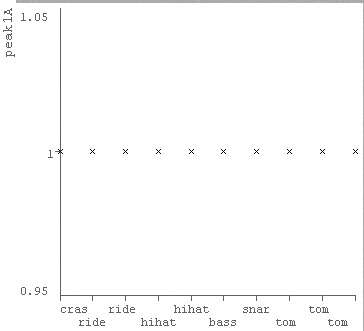
\includegraphics[width=5cm]{images/weka/vis/peak1A.png}
		\label{fig:visPeak1A}
	}
	\subfloat[Peak 2]{
		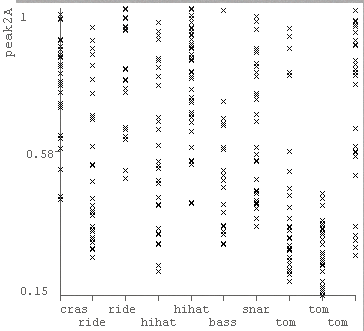
\includegraphics[width=5cm]{images/weka/vis/peak2A.png}
		\label{fig:visPeak2A}
	}
	\subfloat[Peak 3]{
		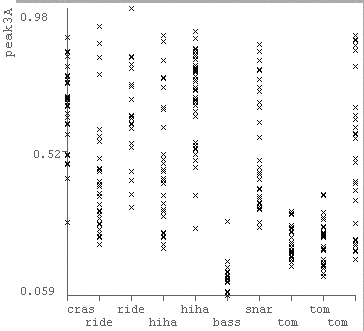
\includegraphics[width=5cm]{images/weka/vis/peak3A.png}
		\label{fig:visPeak3A}
	}
	\caption{Amplitudes of the three maximum peaks.}
	\label{fig:visPeaksA}
\end{figure}

Figure \ref{fig:visPeaksA} shows the distribution of values for the amplitudes of the three maximum peaks. For the maximum peak (figure \ref{fig:visPeak1A}), the value 1 is always returned, because of the normalization of the frequency spectrum, which was described in section \ref{section:method1pre-processing}. Thus, this feature can be discarded for all feature sets. The amplitudes for peak 2 (figure \ref{fig:visPeak2A}) and peak 3 (figure \ref{fig:visPeak3A}) show values between 0 and 1. There are huge overlapping areas in both of the graphics. Furthermore, there are few repeating values. It is observed that the values for the cymbals and the snare drum tend to be placed in higher ranges, whereas the values for the drums are placed in lower ones. For the drums there is mostly just one outstanding peak, which is much higher than the remaining ones. An exception of this example is the tom 3. It shows three maximum peaks of similar height when a loud or edged stroke is done. The values for the ride cymbal, closed hi-hat and tom 3 spread over the entire range of values. Thus, they can't be distinguished with the help of this features. The best results are gained for the ride bell, the bass drum, tom 1 and tom 2. They show values that tend to conglomerate on a specific area. This behavior can help to distinguish between the different class labels. With peak 3, a better differentiation is achieved than with peak 2. Hence, peak 2 is used for feature set 1 and peak 3 for feature set 1 and feature set 2.

The distribution of the maximum peaks frequencies are displayed in figure \ref{fig:visPeaksF}. In contrast to the values for the amplitudes, here are observed many repeating values. This is because the maximum peaks generally rise at the same places for each drum. Thus, the peak frequencies can help to distinguish between the drums if their peak positions are not overlapping. There are observed partially overlapping values for strokes on the ride cymbal and on the ride bell as well as for strokes on the opened and closed hi-hat. The best results are gained for peak 1. For peak 2 and peak 3 the peaks are varying more in their positions. Thus, peak 1 is used for feature sets 1 and feature set 2, peak 2 is only used for feature set 1 and peak 3 is discarded from all feature sets.

%peak frequencies
\begin{figure}[tp]
	\centering
	\subfloat[Peak 1]{
		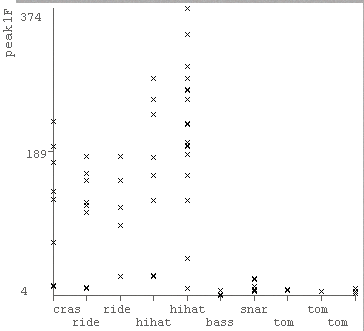
\includegraphics[width=5cm]{images/weka/vis/peak1F.png}
		\label{fig:visPeak1F}
	}
	\subfloat[Peak 2]{
		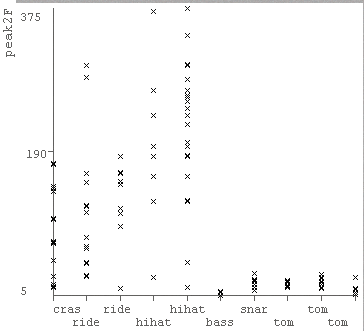
\includegraphics[width=5cm]{images/weka/vis/peak2F.png}
		\label{fig:visPeak2F}
	}
	\subfloat[Peak 3]{
		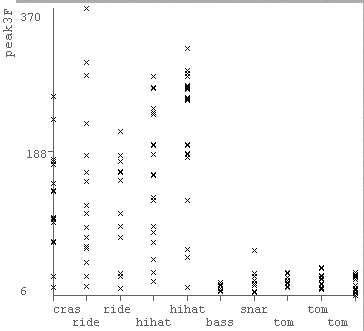
\includegraphics[width=5cm]{images/weka/vis/peak3F.png}
		\label{fig:visPeak3F}
	}
	\caption{Frequencies of the three maximum peaks.}
	\label{fig:visPeaksF}
\end{figure}


The further features, which are based on the peaks in the frequency spectrum, are displayed in figure \ref{fig:visPeakFeatures}. These are the number of peaks (figure \ref{fig:visMeanPeakF}) and the mean peak amplitude (figure \ref{fig:visMeanPeakA}) and frequency (figure \ref{fig:visMeanPeakF}). For most values these features show a conglomeration of peaks for the different class labels.

The number of peaks is much higher for the cymbals and snare drum than for the other drums. The cymbal with the lowest number of peaks is the ride bell and the one with the most peaks is the closed hi-hat. They can be clearly separated from each other. Moreover, the drums (except for the snare drum) can be clearly separated from the cymbals because of their low values. It can be clearly separated between bass drum, snare drum and toms, but not between the different toms. The lowest values are reached for the bass drum, the highest ones for the snare drum. The values for the three toms are located between snare and bass drum. Hence, the number of peaks provides a good feature to differentiate between most class labels, which is why it is used in all of the feature sets.

The mean peak amplitude shows an explicit difference between the bass drum and the other drums and cymbals. Here, the amplitude is much higher and can be clearly separated from the other drums in the majority of cases. In fewer cases, the values can overlap with the values of tom 3. The three toms have similar ranges, whereof tom 2 has the smallest range and tom 3 the largest. If the toms are compared with the snare drum, it is observed that the snare drum mostly has a lower mean amplitude and thus can be distinguished from the toms for most instances. The cymbals show overlapping, only slightly varying ranges. Thus, they can hardly be separated by this feature. Hence, the mean peak amplitude is used for feature set 1 and feature set 2.   

The mean peak frequency can help to distinguish between most of the drums. Here the ranges for the cymbals also show differences and are only overlapping in some parts. Merely for the opened hi-hat, the values spread over almost the whole range of values. For the cymbals there is a good differentiation between the snare drum, the bass drum and the toms, but the value range for the different toms is overlapping again. Hence, the mean peak frequency is used for all feature sets.

%number of peaks, mean peak amplitude, frequency
\begin{figure}[tp]
	\centering
	\subfloat[Number of peaks]{
		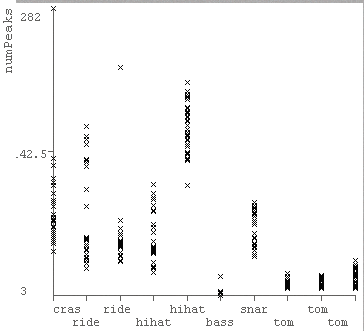
\includegraphics[width=5cm]{images/weka/vis/numPeaks.png}
		\label{fig:visNumPeaks}
	}
	\subfloat[mean peak amplitude]{
		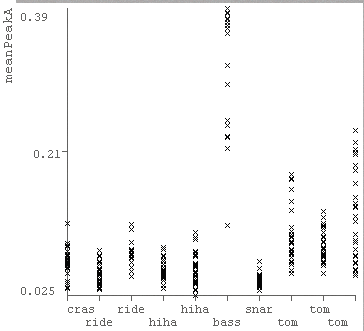
\includegraphics[width=5cm]{images/weka/vis/meanPeakA.png}
		\label{fig:visMeanPeakA}
	}
	\subfloat[mean peak frequency]{
		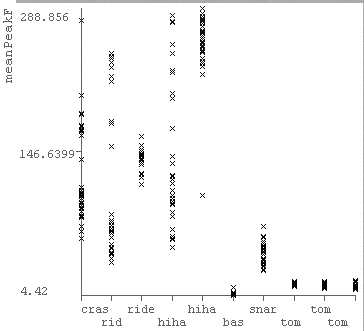
\includegraphics[width=5cm]{images/weka/vis/meanPeakF.png}
		\label{fig:visMeanPeakF}
	}
	\caption{Features extracted from the peaks in the spectrum.}
	\label{fig:visPeakFeatures}
\end{figure}

For the quadratic mean, which is displayed in figure \ref{fig:visMeanA}, also parallels in the value ranges for the particular class labels can be observed. The cymbals show very similar ranges. Merely the closed hi-hat shows higher values than the other cymbals, but is also overlapping with them. For the drums, the snare drum and the tom 3 are overlapping, as well as tom 1 and tom 2 and the bass drum. In contrast to the preceding features, tom 3 can be differentiated  from the other toms in most of the cases. The feature is used for feature set 1 and feature set 2.

%Mean amplitude %mean frequency
\begin{figure}[tp]
	\centering
	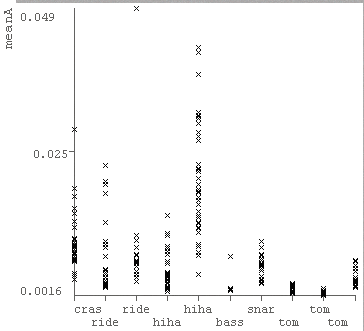
\includegraphics[width=5cm]{images/weka/vis/meanA.png}
	\label{fig:visMeanA}
	\caption{Quadratic mean energy of the entire spectrum.}
	\label{fig:visMeanA}
\end{figure}

Next, the different features extracted from the two intervals from 0 Hz to 2000 Hz (interval 1) and from 2000 Hz to 22.050 Hz (interval 2) are considered. These features are the maximum peak amplitude and frequency of interval 1 (figures \ref{fig:visMaxAI1} and \ref{fig:visMaxFI1}), the mean amplitude of interval 1 and interval 2 (figures \ref{fig:visMeanAI1} and \ref{fig:visMeanAI2}) and the interval rate (figure \ref{fig:visIRate}).

Like the maximum peak amplitude of the entire spectrum, the values for interval 1 are usually one, because of the normalization. Only for the cymbals, where the maximum peak is placed within interval 2, the values are lower. The values varying from one are spread over the entire value range. Thus, the feature is discarded for all feature sets. The maximum peak frequency shows a similar result to the ones of the entire spectrum. If only the value in interval 1 is considered, there are less possible peak values, which can improve the result. Furthermore, there are less overlapping values and the calculation time for the feature is lower. Thus, the feature is used for every feature set.

%intervals max peaks
%intervals mean peaks, interval rate
\begin{figure}[tp]
	\centering
	\subfloat[Maximum peak amplitude of interval 1]{
		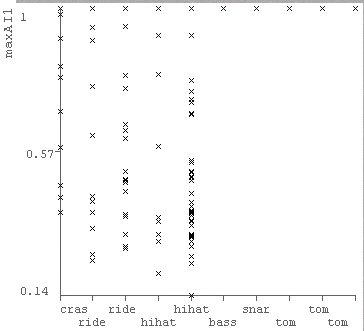
\includegraphics[width=5cm]{images/weka/vis/maxAI1.png}
		\label{fig:visMaxAI1}
	}
	\subfloat[Maximum peak frequency of interval 1]{
		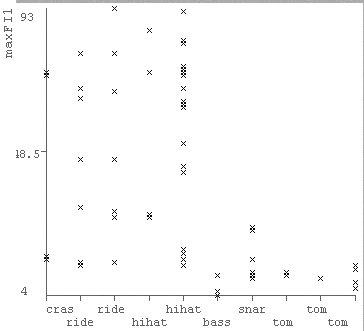
\includegraphics[width=5cm]{images/weka/vis/maxFI1.png}
		\label{fig:visMaxFI1}
	}
	\caption{Maximum peak extracted from interval 1 (0-2000 Hz)}
	\label{fig:visIntervalFeatures1}
\end{figure}

The quadratic mean amplitude of interval 1 (figure \ref{fig:visMeanAI1}) shows few differences between the cymbals. For the drums there are also overlapping ranges, which are equal to the quadratic mean energy of the entire spectrum. Since the cymbals can be differentiated better by considering the entire spectrum, the quadratic mean amplitude of interval 1 feature is only used for feature set 1. For interval 2, the quadratic mean is more significant for the cymbals. The ride cymbal and the opened hi-hat show the lowest values. The values of the crash cymbal and the ride bell are overlapping with their range, but start with higher values. The closed hi-hat shows even higher values. The range of its values is much wider than the range of the other cymbals. Some of the values are overlapping, but most values can be differentiated. The drums show much lower values than the cymbals due to their absence of peaks in this frequency range. Only the snare drum shows some outstanding values, which are similar to the values of the opened hit-hat and the ride cymbal. Thus, the snare drum can be differentiated from the recent drums. As the bass drum and the toms show the same value ranges, they cannot be differentiated from each other. Hence, the feature is used for feature set 1 and feature set 2.

The interval rate shows similar characteristics to the quadratic mean amplitude with inverted value ranges. This is due to the fact that the values of the quadratic mean in interval 2 are smaller than the ones in interval 1. Thus, they are carrying almost no weight, except to invert the values to negative ones. Hence, the feature is discarded for all feature sets.

\begin{figure}[tp]
	\centering
	\subfloat[Quadratic mean amplitude of interval 1]{
		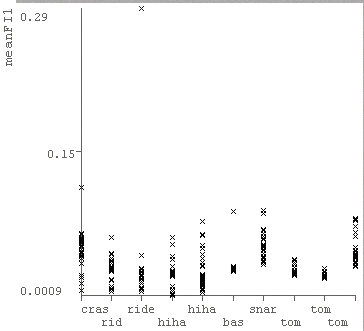
\includegraphics[width=5cm]{images/weka/vis/meanAI1.png}
		\label{fig:visMeanAI1}
	}
	\subfloat[Quadratic mean amplitude of interval 2]{
		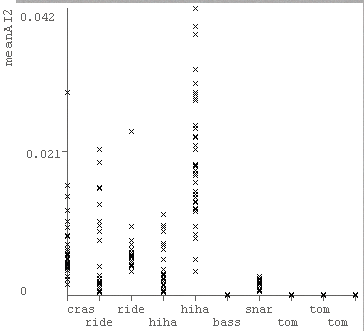
\includegraphics[width=5cm]{images/weka/vis/meanAI2.png}
		\label{fig:visMeanAI2}
	}
	\subfloat[Interval rate]{
		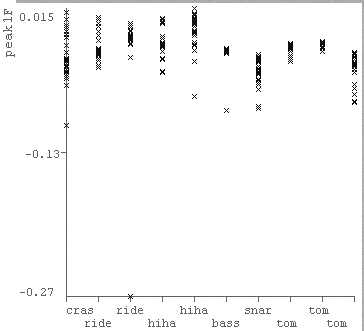
\includegraphics[width=5cm]{images/weka/vis/irate.png}
		\label{fig:visIRate}
	}
	\caption{Mean amplitudes and interval rate of interval 1 (0-2000 Hz) and interval 2 (2001-22.050 Hz).}
	\label{fig:visIntervalFeatures2}
\end{figure}

Next, the features based on the three subsequent frames are analyzed. These are the maximum peak amplitudes and frequencies of each of the frames (figure \ref{fig:visFramePeaks}) as well as the maximum and the mean steadiness (figure \ref{fig:visS}).

The maximum peak amplitudes for the three frames show largely overlapping ranges. The value ranges of the cymbals are similar in each frame. Most of their values are overlapping and thus cannot be differentiated. The values for the drums show varying ranges. Two clusters for each drum, formed due to the different stroke intensities, are observed. Low and high powered sounds are trained, so it can be assumed that the area between the two clusters would be filled by medium powered strokes. Hence, the ranges for the drum would also be overlapping and would not be significant enough for a differentiation. Therefore, the maximum peak amplitudes of the frames are not used for the feature sets.

The maximum peak frequencies of the three frames show similar characteristics to the maximum peak frequency of the single frame, differing in the positions of the peaks. The positions of peaks are also different between the three frames. The features are used for feature set 1. Additionally, the maximum peak frequency for the second window is used for feature set 2.

%frames peaks
\begin{figure}[tp]
	\centering
	\subfloat[Maximum peak amplitude of frame 1]{
		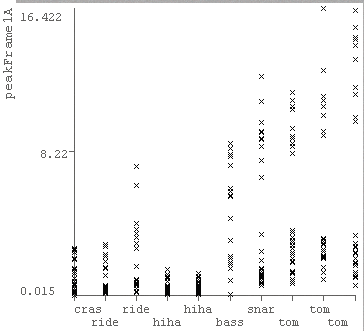
\includegraphics[width=5cm]{images/weka/vis/frame1A.png}
		\label{fig:visFrame1A}
	}
	\subfloat[Maximum peak amplitude of frame 2]{
		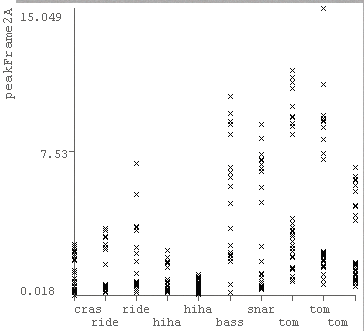
\includegraphics[width=5cm]{images/weka/vis/frame2A.png}
		\label{fig:visFrame2A}
	}
	\subfloat[Maximum peak amplitude of frame 3]{
		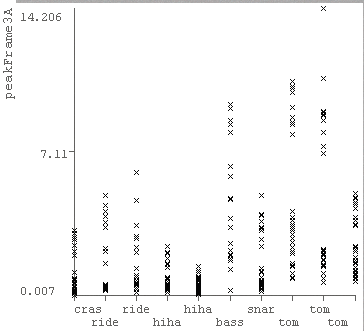
\includegraphics[width=5cm]{images/weka/vis/frame3A.png}
		\label{fig:visFrame3A}
	}
	\qquad
	\subfloat[Maximum peak frequency of frame 1]{
		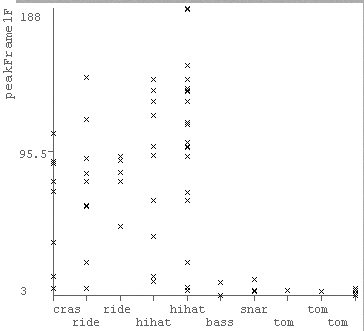
\includegraphics[width=5cm]{images/weka/vis/frame1F.png}
		\label{fig:visFrame1F}
	}
	\subfloat[Maximum peak frequency of frame 2]{
		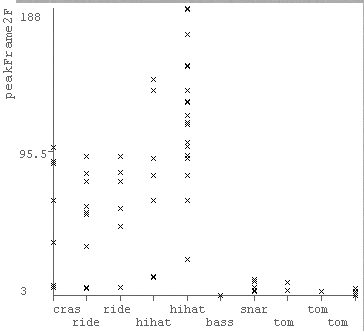
\includegraphics[width=5cm]{images/weka/vis/frame2F.png}
		\label{fig:visFrame2F}
	}
	\subfloat[Maximum peak frequency of frame 3]{
		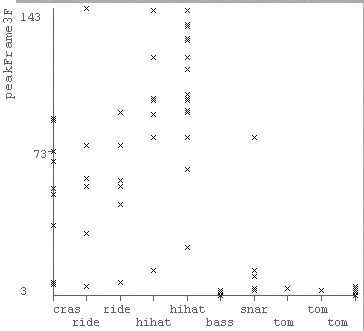
\includegraphics[width=5cm]{images/weka/vis/frame3F.png}
		\label{fig:visFramePeaks}
	}
\end{figure}


The resulting values for the steadiness of the maximum peak are overlapping in a wide range for most class labels. The values for the crash cymbal and the opened hi-hat vary most. They spread over the entire value range. The best results are gained for the toms. Tom 1 and tom 2 only show very low values, whereas tom 3 produces mainly centered and some high values. There is one outlier which is placed in the same range as tom 1 and tom 2. The maximum peaks steadiness is used for feature set 1.

The mean steadiness shows more differentiating but also overlapping ranges than the steadiness of the maximum peak. The ranges of the different class labels have a similar dimension. Merely the crash cymbal spreads over the entire value range, whereby it tends to produce low and centered values. The cymbals are widely overlapping, except of the closed hi-hat, which shows much higher values. The drums, the bass drum, the snare drum and tom 3 show higher values than tom 1 and tom 2. Their ranges are also widely overlapping. The mean steadiness is used for feature set 1 and feature set 2.

%steadiness
\begin{figure}[tp]
	\centering
	\subfloat[Steadiness of maximum peak]{
		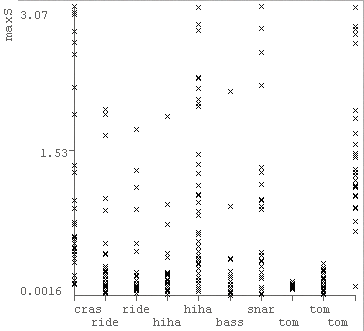
\includegraphics[width=5cm]{images/weka/vis/maxS.png}
		\label{fig:visMaxS}
	}
	\subfloat[Mean steadiness]{
		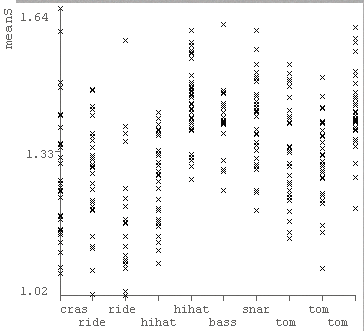
\includegraphics[width=5cm]{images/weka/vis/meanS.png}
		\label{fig:visMeanS}
	}
	\caption{Features based on the steadiness.}
	\label{fig:visS}
\end{figure}

\newpage
For each feature set, there is created a Weka .arff training file containing the training data and a test file containing the test data.

In the training sets are 696 instances (24 for each trained stroke type) and in the test set are 290 instances (ten for each trained stroke type). There is no differentiation between the stroke types for a particular drum or cymbal.

Feature set 1 uses the following relation on the basic .csv training and test data files:

\lstinline{data-weka.filters.unsupervised.attribute.Remove-R3,6,13-14,17,19,21,23}

Hence, the following 17 attributes remain:

\begin{itemize} 
	\item drums
	\item peak 1 (frequency)
	\item peak 2 (frequency)
	\item peak 2 (amplitude)
	\item peak 3 (amplitude)
	\item number of peaks
	\item mean peak (frequency)
	\item mean peak (amplitude)
	\item mean amplitude
	\item maximum peak interval 1 (frequency)
	\item mean amplitude interval 1
	\item mean amplitude interval 2
	\item peak frame 1 (frequency)
	\item peak frame 2 (frequency)
	\item peak frame 3 (frequency)
	\item maximum steadiness
	\item mean steadiness	
\end{itemize}

Feature set 2 uses the following relation on the basic .csv training and test data files:

\lstinline{data-weka.filters.unsupervised.attribute.Remove-R3-6,13-15,17-19,21-24}

The following eleven attributes remain:

\begin{itemize} 
	\item drums 1
	\item peak 1 (frequency)
	\item peak 3 (amplitude)
	\item number of peaks
	\item mean peak (frequency
	\item mean peak (amplitude)
	\item mean amplitude
	\item maximum peak interval 1 (frequency)
	\item mean amplitude interval 2
	\item peak frame 2 (frequency)
	\item mean steadiness	
\end{itemize}

Feature set 3 uses the following relation on the basic .csv training and test data files:

\lstinline{data-weka.filters.unsupervised.attribute.Remove-R2-7,10-11,13-25}

The following four attributes remain:

\begin{itemize} 
	\item drums
	\item number of peaks
	\item mean peak (frequency)
	\item maximum peak interval 1 (frequency)
\end{itemize}

The attribute \textit{drums} is the nominal value that defines the class labels for the particular drums and cymbals.

\subsubsection{Classification in Weka}

%Mit Hilfe von Weka kann das mit dem Feature Extractor erstellte Textfile analysiert werden.
%Um zusätzlich zur Unterscheidung zwischen den einzelnen Drums und Cymbals auch unterscheiden zu können, ob es sich um eine Trommel oder ein Becken handelt, wird dem Textfile manuell eine Spalte hinzugefügt, die dieses angibt. Außerdem wurde je ein zusätzliches File erstellt, in dem nur Trommeln bzw. nur Becken enthalten sind.
%Das File wird anschließend in Weka geladen. Hier werden alle nicht benötigten Features gelöscht. Anschließend können verschiedene Klassifikationsalgorithmen auf die Daten angewand werden. Dabei stellt sich heraus, dass die in Weka enthaltenen Algorithmen 'J48 Tree' und 'Simple Card' die besten Ergebnisse liefern.
%Verwendete Einstellungen
%Für die erste Analyse in Weka wurden Audiofiles mit 44.100 Hz aufgenommen. Jede Drum / jedes Becken wurde 20 mal mit verschiedenen Schlagintensitäten eingespielt. Das Mikrofon wurde dabei über dem Schlagzeug platziert. Im Feature Extractor wurde eine Framesize von 1024 für die drei aufeinanderfolgenden Frames ausgewählt. Daraus ergibt sich eine Framesize von 3072 für den nicht unterteilten Frame.

The developed feature sets are used for the classification in Weka. The pruned C4.5 decision tree using the J48 algorithm in Weka, is chosen as the classification algorithm. The algorithm is trained with the training data file. As test set, the test data file is applied. As parameters for the algorithm, the standard parameters of Weka are used. These are a confidence factor of 0.25 and a minimum number of instances per leaf of 2. The confidence factor is used for pruning, whereby smaller values incur more pruning. The used Weka scheme is \lstinline{weka.classifiers.trees.J48 -C 0.25 -M 2}.


\subsubsection{Results Feature Set 1}

For feature set 1, the tree displayed in figure \ref{fig:wekaTree1} is gained. It shows a size of 37 nodes, a height of nine and a number of 19 leaves. The classification system is built in 0.22 seconds. There are 243 correctly classified and 47 incorrectly classified instances, which equals a hit-rate of 83.79 \%. Tables \ref{tab:WekaEval1} and \ref{tab:wekaAcc1} show a summary for the evaluation of the test set with feature set 1 and a detailed accuracy by class.

\begin{figure}[h]
	\centering
  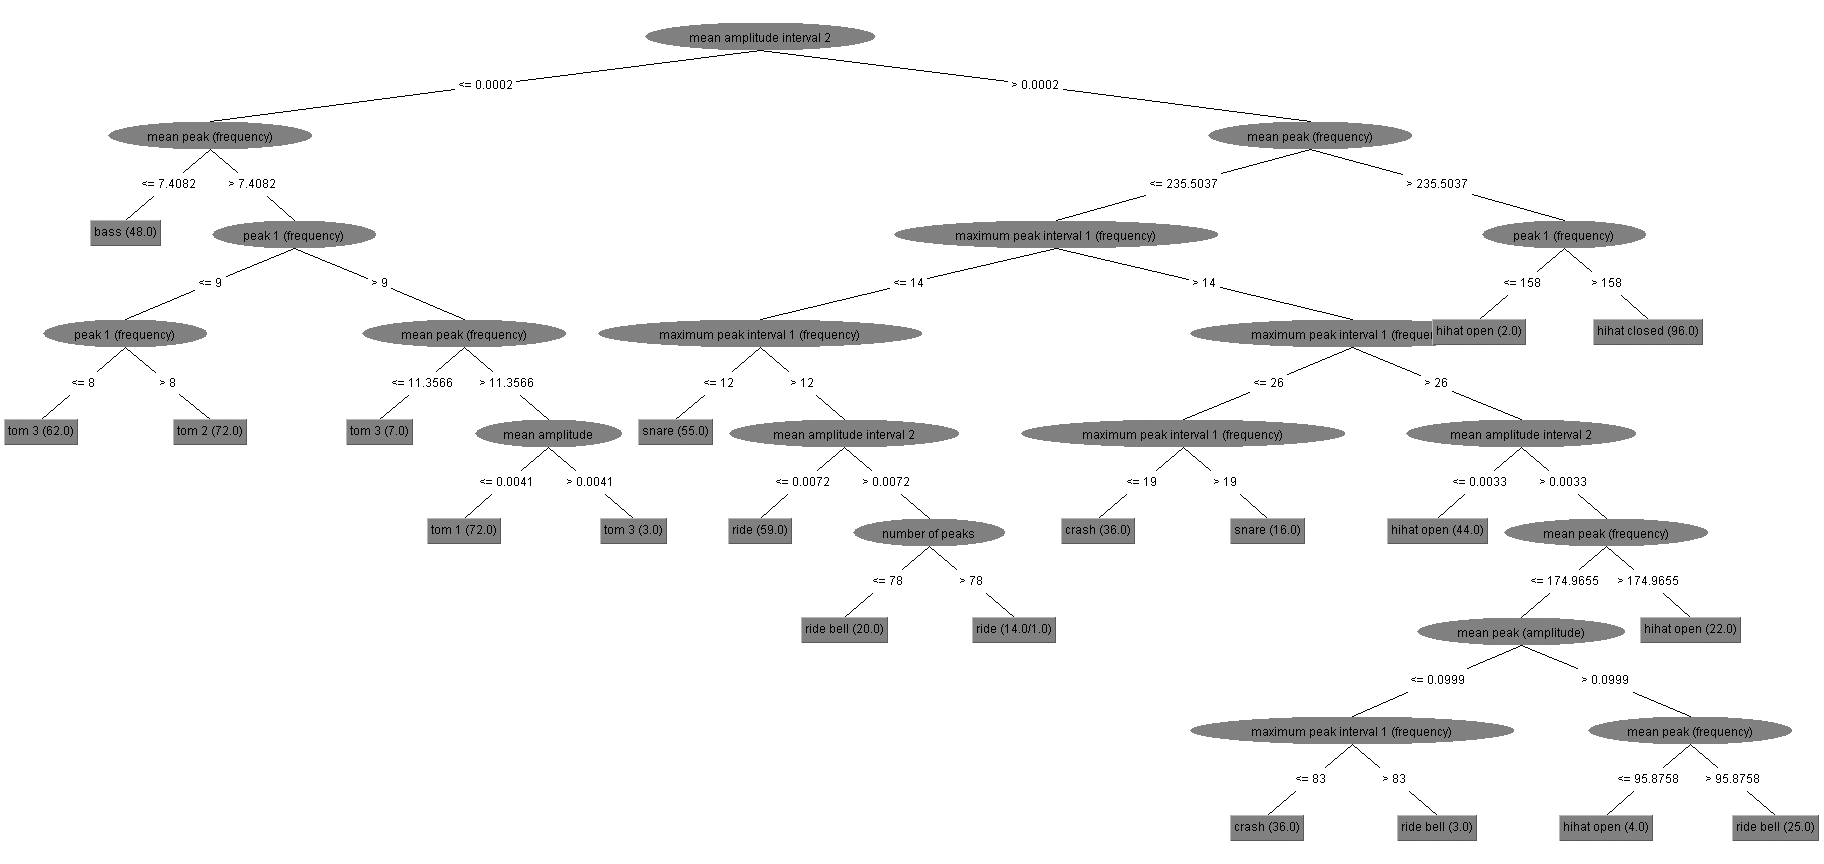
\includegraphics[width=\textwidth]{images/weka/weka_tree_1.png}
	\caption{J48 tree of feature set 1.}
	\label{fig:wekaTree1}
\end{figure}

\begin{table}[h]
  \caption{Evaluation on feature set 1}
  \label{tab:WekaEval1} 
	\centering
	\footnotesize
	\begin{tabular}[c]{|l|l|}
	  \hline
		Correctly Classified Instances & 243 (83.7931 \%) \\
	  \hline
		Incorrectly Classified Instances & 47 (16.2069 \%) \\
	  \hline
		Kappa statistic & 0.819  \\
	  \hline
		Mean absolute error & 0.0329 \\
	  \hline
		Root mean squared error & 0.1797 \\
	  \hline
		Relative absolute error & 18.3462 \% \\
	  \hline
		Root relative squared error & 60.0304 \% \\
	  \hline
		Total Number of Instances & 290  \\
	  \hline
	\end{tabular}
\end{table}

\begin{table}
  \caption{Detailed accuracy by class for feature set 1}
  \label{tab:wekaAcc1} 
	\centering
	\footnotesize
	\begin{tabular}[c]{|l|l|l|l|l|l|l|l|}
	  \hline
		& TP Rate &  FP Rate &  Precision  & Recall & F-Measure  & ROC Area & Class \\
	  \hline
    & 0.933 & 0.065    &  0.622  &   0.933  &   0.747   &   0.91  &  crash \\
	  \hline
    & 0.667 &   0.015  &    0.833   &  0.667  &   0.741  &    0.827  &  ride \\
	  \hline
    &  0.4 &    0.004  &    0.889  &   0.4    &   0.552  &    0.698  &  ride bell \\
	  \hline
    & 0.7 &   0.062  &    0.568 &    0.7    &   0.627  &    0.819  &  hihat open \\
	  \hline
    & 0.775 &   0.028  &    0.816 &    0.775  &   0.795 &     0.874 &   hihat closed \\
	  \hline
    & 0.95 &    0      &    1    &     0.95   &   0.974 &     0.975 &   bass \\
	  \hline
    &  0.867 &   0.004  &    0.963 &    0.867 &    0.912 &     0.94 &    snare \\
	  \hline
    & 1 &     0     &     1     &    1     &    1     &     1    &    tom 1 \\
	  \hline
    & 1 &      0     &     1     &    1    &     1    &      1    &    tom 2 \\
	  \hline
    & 1 &      0.004   &   0.968  &   1    &     0.984  &    0.998 &   tom 3 \\
	  \hline
Weighted Avg.   & 0.838 &    0.02   &   0.859  &   0.838  &   0.837   &   0.908  & \\
	  \hline
	\end{tabular}
\end{table}

\newpage
The resulting confusion matrix, which is displayed in figure \ref{fig:wekaMatrix1} shows how the test records are classified. The correctly classified instances are colored in green, the incorrectly classified instances in red. 

\begin{figure}[tp]
	\centering
  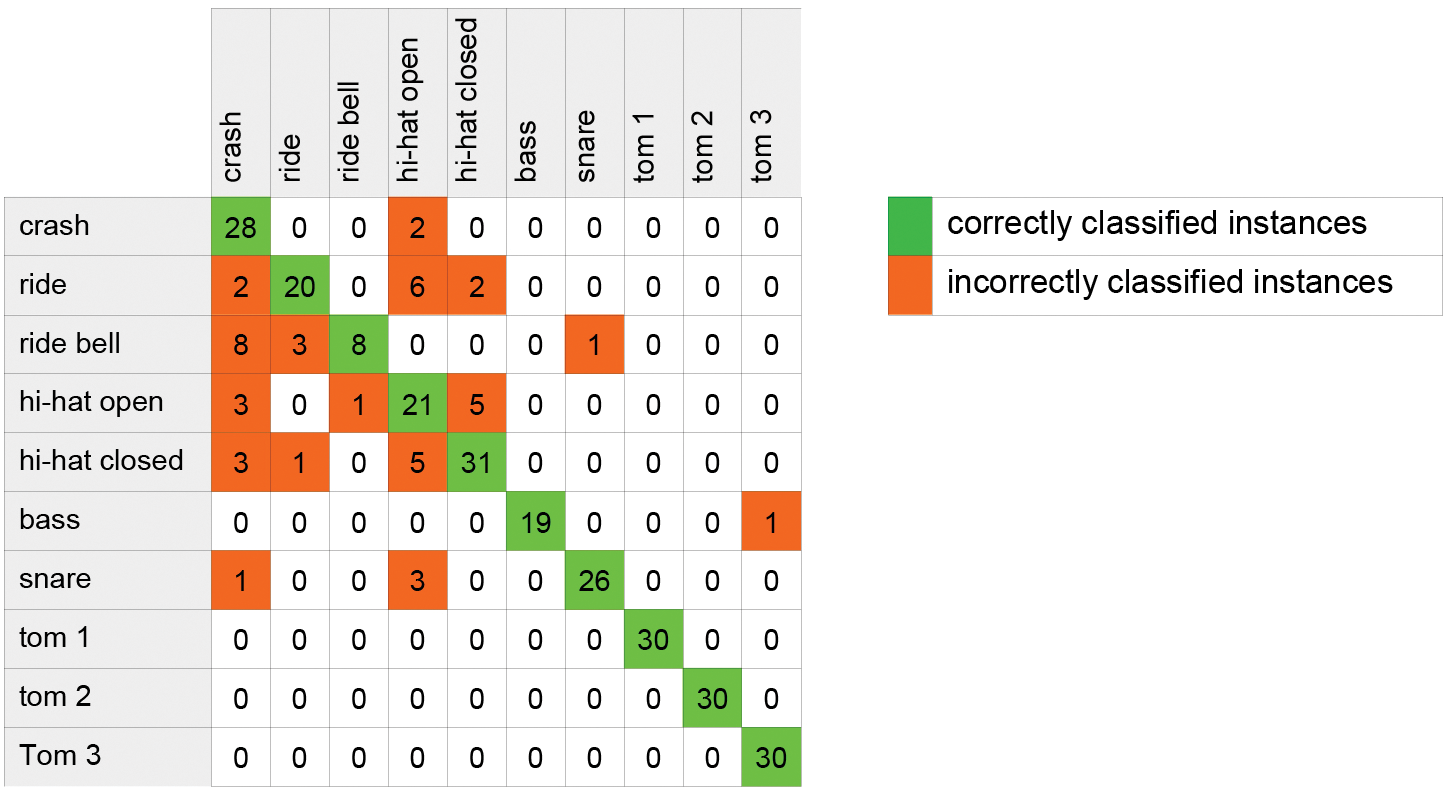
\includegraphics[width=.65\textwidth]{images/weka/weka_matrix_1.png}
	\caption{Confusion Matrix for J48 tree on feature set 1.}
	\label{fig:wekaMatrix1}
\end{figure}

For the cymbals, there are 108 correctly classified instances out of a total of 150 instances. For the drums there are 135 out of 140 instances classified with the right class label. Thus, the hit-rate for the cymbals is 72 \% and the hit-rate for the drums 96.43 \%. The highest hit-rate is received for the tom toms. Each of them shows a hit-rate of 100 \%. The bass drum shows only one wrong classified instance, which is declared as a tom 3. The snare drum shows four errors out of 30 instances. It is falsely classified once as the crash cymbal, and three times as the opened hi-hat. The highest number of misses is gained for the ride bell. Here, twelve out of 20 records are classified incorrectly. 8 instances with the class label for the ride bell are classified as crash cymbal, three as ride cymbal and one as snare. The best results for the cymbals are gained for the crash drum. Here, only two incorrectly classified instances are received. These two instances are classified as the opened hi-hat. Furthermore, the ride cymbal shows ten errors out of 30 instances, the opened hi-hat nine errors out of 30 instances and the closed hi-hat shows nine errors out of 40 test instances.

\subsubsection{Results Feature Set 2}

For feature set 2, the tree displayed in figure \ref{fig:wekaTree2} is gained. It shows a size of 39 nodes, a height of nine and a number of 20 leaves. The classification system is built in 0.2 seconds. There are 247 correctly classified and 47 incorrectly classified instances, which equals a hit-rate of 85.17 \%. Thus, the hit-rate is improved by 1.38 \% in contrast to feature \linebreak set 1. Tables \ref{tab:WekaEval2} and \ref{tab:wekaAcc2} show a summary for the evaluation on the test set with feature set 1 and a detailed accuracy by class.

\begin{figure}[bp]
	\centering
  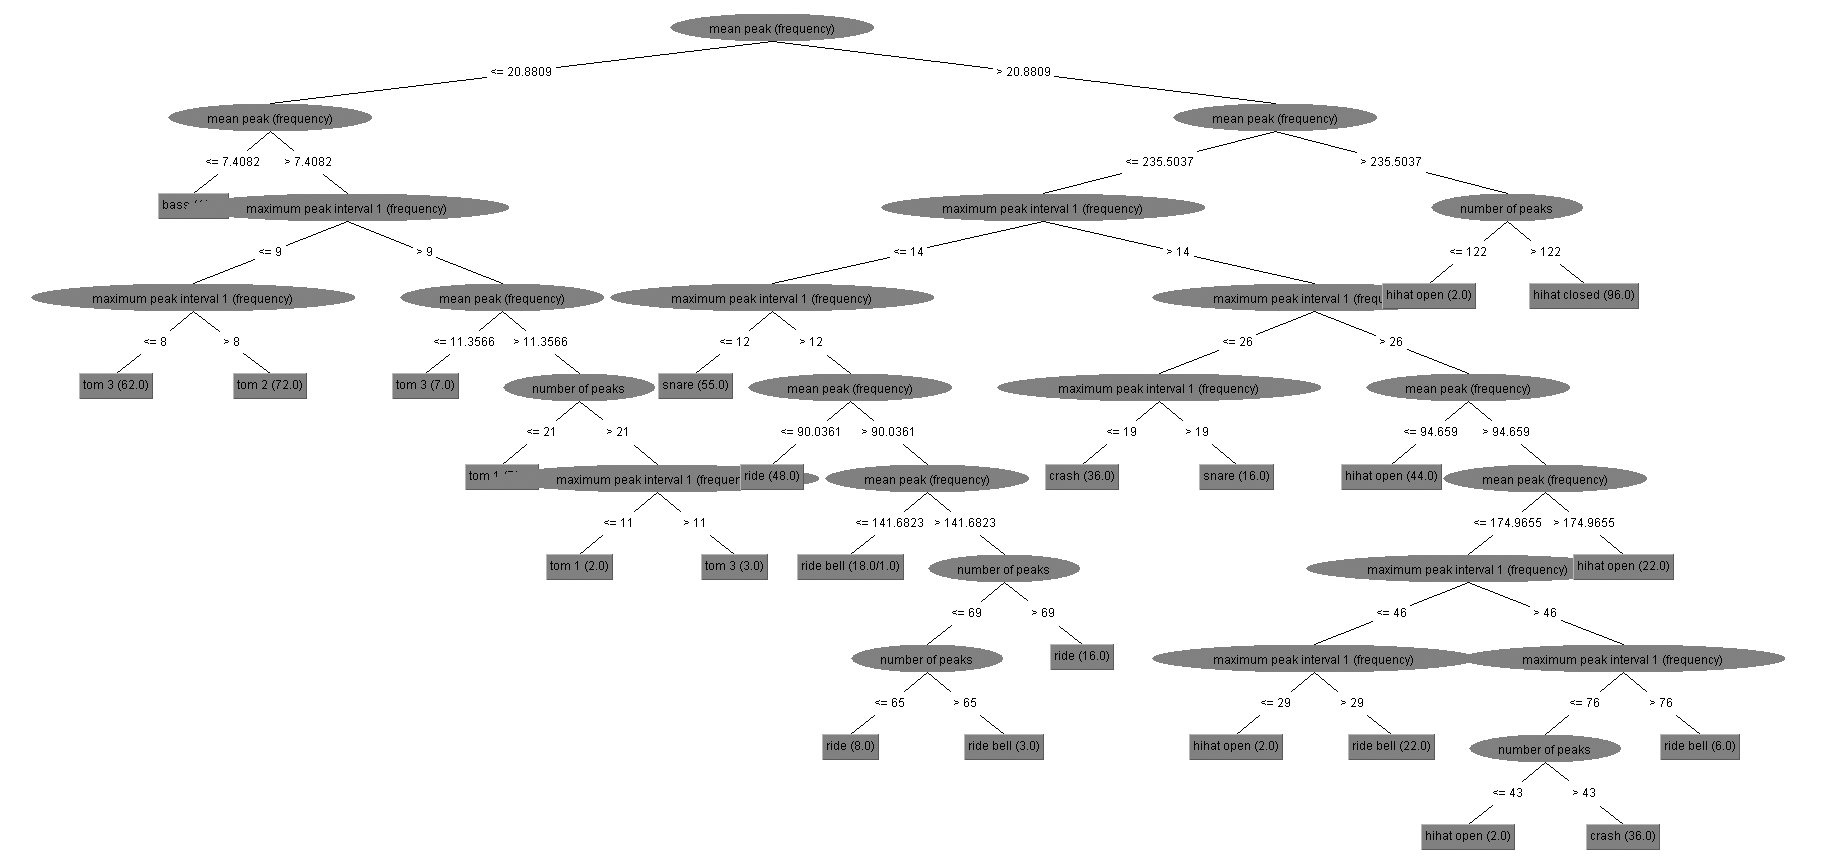
\includegraphics[width=\textwidth]{images/weka/weka_tree_2.png}
	\caption{J48 tree of feature set 2.}
	\label{fig:wekaTree2}
\end{figure}

\begin{table}[bp]
  \caption{Evaluation on feature set 2}
  \label{tab:WekaEval2} 
	\centering
	\footnotesize
	\begin{tabular}[c]{|l|l|}
	  \hline
		Correctly Classified Instances   &      247 (85.1724 \%) \\
	  \hline
Incorrectly Classified Instances    &    43 (14.8276 \%) \\
	  \hline
Kappa statistic      &                    0.8344 \\
	  \hline
Mean absolute error    &                  0.0297 \\
	  \hline
Root mean squared error  &                0.1721 \\
	  \hline
Relative absolute error  &               16.5376 \% \\
	  \hline
Root relative squared error   &          57.4681 \% \\
	  \hline
Total Number of Instances    &          290   \\
	  \hline
	\end{tabular}
\end{table}

\begin{table}[bp]
  \caption{Detailed accuracy by class for feature set 2}
  \label{tab:wekaAcc2} 
	\centering
	\footnotesize
	\begin{tabular}[c]{|l|l|l|l|l|l|l|l|}
	  \hline
		   &            TP Rate &  FP Rate & Precision &  Recall  &F-Measure &  ROC Area & Class \\
	  \hline
      &           0.933  &   0.065   &   0.622  &   0.933  &   0.747   &   0.934   & crash \\
	  \hline
        &         0.667  &   0.015    &  0.833  &   0.667   &  0.741   &   0.827   & ride \\
	  \hline
        &         0.45   &   0.004   &   0.9    &   0.45   &   0.6    &    0.723  &  ride bell \\
	  \hline
        &         0.7    &   0.05   &    0.618  &   0.7    &   0.656    &  0.825 &   hihat open \\
	  \hline
       &          0.775  &   0.028  &    0.816  &   0.775  &   0.795    &  0.874 &   hihat closed \\
	  \hline
       &          0.95   &   0    &      1   &      0.95   &   0.974    &  0.975  &  bass \\
	  \hline
       &          0.967  &   0    &      1    &     0.967   &  0.983    &  0.983 &   snare \\
	  \hline
       &          1    &     0   &       1     &    1    &     1    &      1     &   tom 1 \\
	  \hline
       &          1   &     0    &      1      &   1    &     1    &      1    &    tom 2 \\
	  \hline
       &          1  &       0.004    &  0.968   & 1   &      0.984    &  0.998   & tom 3 \\
	  \hline
Weighted Avg. &   0.852   &  0.018  &    0.868  &   0.852   &  0.85  &     0.917  & \\
	  \hline
	\end{tabular}
\end{table}

The confusion matrix for feature set 2 is displayed in figure \ref{fig:wekaMatrix2}. For the cymbals, there are 109 correctly classified instances out of a total of 150 instances for cymbals. Thus, there is one hit more than for feature set 1. For the drums there are 138 out of 140 instances classified with the right class label, which is an increase of three hits in contrast to feature set 1. In terms of a percentage, the hit-rate for the cymbals is 72.66 \% and the hit-rate for the drums 98.57 \%. This means an increase of 0.66 \% for the cymbals and 2.14 \% for the drums. 

Hence, the confusion matrix shows similar results as the one for feature set 1. The additional hit for the cymbals is for the test instance of the ride bell, which was declared as snare drum before. The three additional hits for the drums are received for the snare drum. Thus, there is only one miss for this drum, which is classified as crash cymbal.

\begin{figure}[htb]
	\centering
  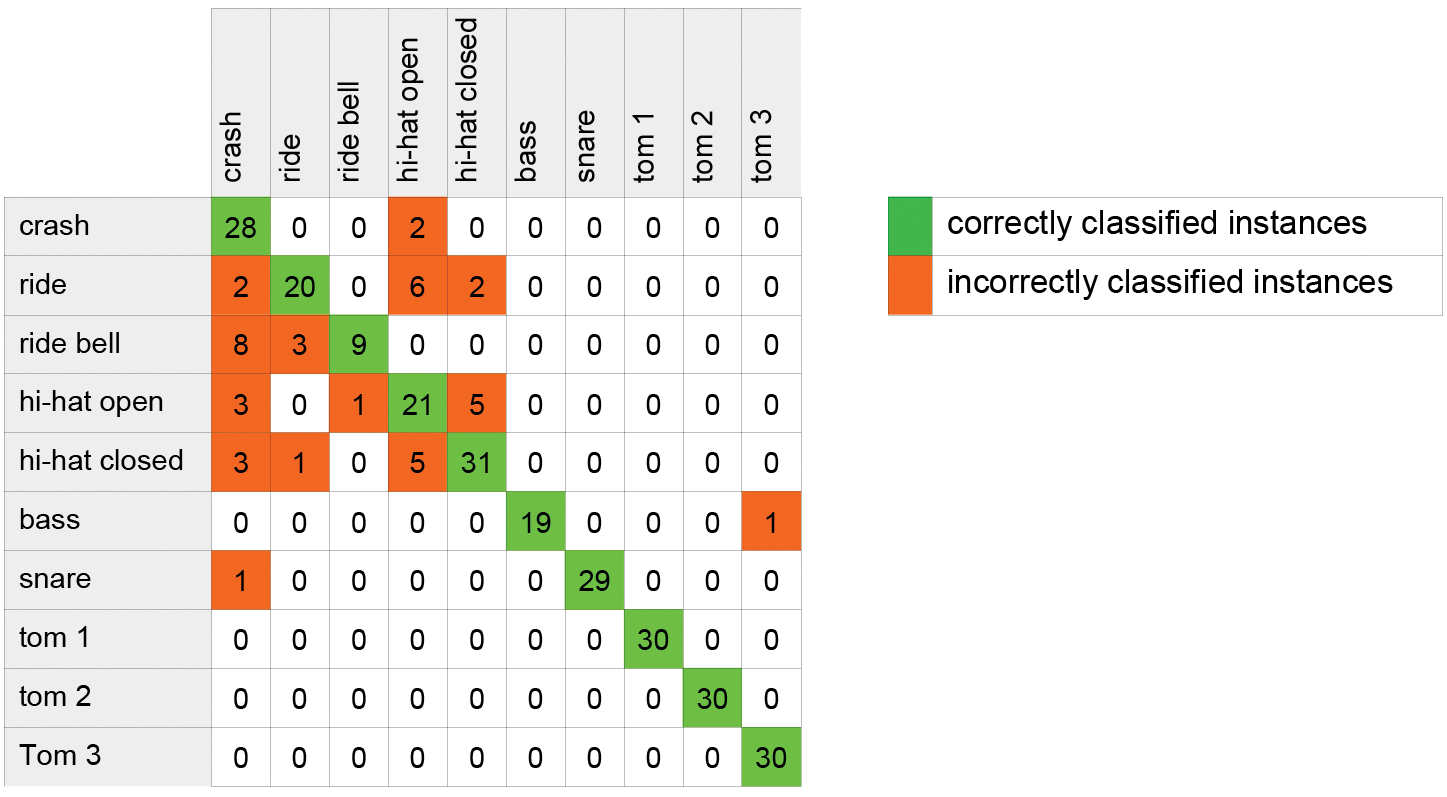
\includegraphics[width=.65\textwidth]{images/weka/weka_matrix_2.png}
	\caption{Confusion Matrix for J48 tree on feature set 2.}
	\label{fig:wekaMatrix2}
\end{figure}


\subsubsection{Results Feature Set 3}

For feature set 3, the tree displayed in figure \ref{fig:wekaTree2} is gained. It shows a size of 47 nodes, a height of ten and a number of 24 leaves. The classification system is built in 0.22 seconds. There are 243 correctly classified and 47 incorrectly classified instances, which equals a hit-rate of 91.72 \%. Thus, the hit-rate is improved by 7.93 \% in contrast to feature set 1 and 6,55 \% in contrast to feature set 2. Tables \ref{tab:WekaEval3} and \ref{tab:wekaAcc3} show a summary for the evaluation on the test set with feature set 1 and a detailed accuracy by class.

\begin{figure}[htb]
	\centering
  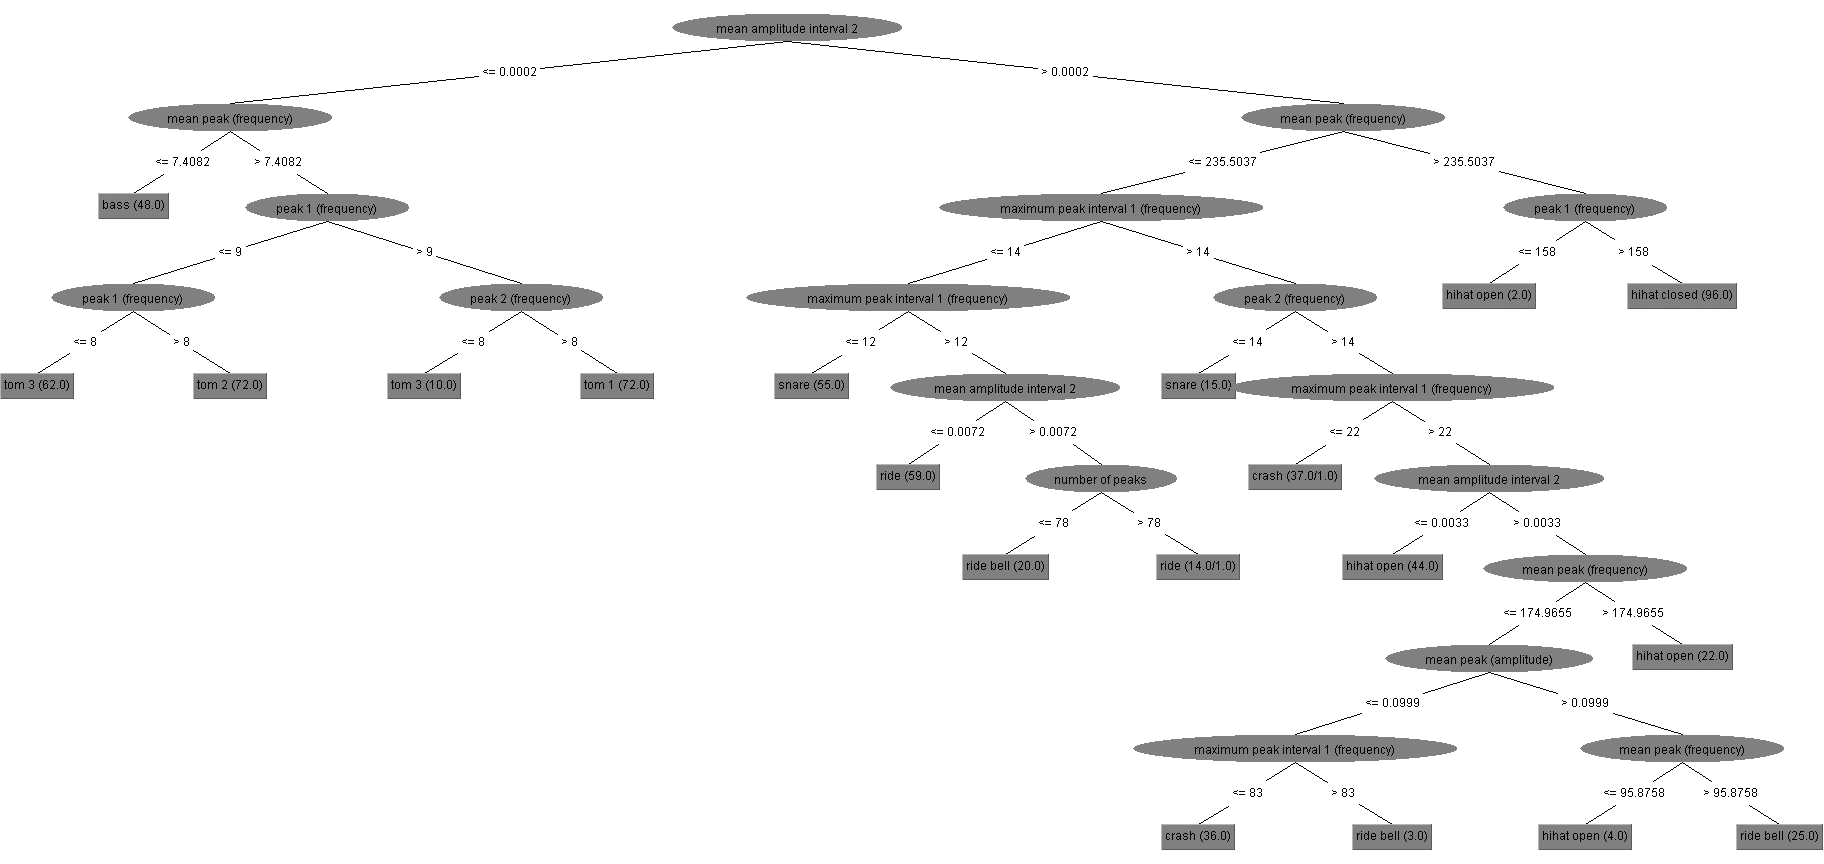
\includegraphics[width=\textwidth]{images/weka/weka_tree_3.png}
	\caption{J48 tree of feature set 3.}
	\label{fig:wekaTree3}
\end{figure}

\begin{table}
  \footnotesize
  \caption{Evaluation on feature set 3}
  \label{tab:WekaEval3} 
	\centering
	\begin{tabular}[c]{|l|l|}
	  \hline
		Correctly Classified Instances   &     266 (91.7241 \%) \\
	  \hline
Incorrectly Classified Instances    &    24 (8.2759 \%) \\
	  \hline
Kappa statistic      &                    0.9077 \\
	  \hline
Mean absolute error    &                  0.0166 \\
	  \hline
Root mean squared error  &                0.1287 \\
	  \hline
Relative absolute error  &               9.273 \% \\
	  \hline
Root relative squared error   &          42.9724 \% \\
	  \hline
Total Number of Instances    &          290 \\
	  \hline
	\end{tabular}
\end{table}

\begin{table}
  \caption{Detailed accuracy by class for feature set 3}
  \label{tab:wekaAcc3} 
	\centering
	\footnotesize
	\begin{tabular}[c]{|l|l|l|l|l|l|l|l|}
	  \hline		  
         &      TP Rate &  FP Rate &  Precision  & Recall &  F-Measure  & ROC Area  &Class \\
	  \hline
          &       0.933  &   0.015   &   0.875  &   0.933   &  0.903   &   0.959   & crash \\
	  \hline
        &         0.667  &   0.008   &   0.909  &   0.667   &  0.769  &    0.829  &  ride \\
	  \hline
        &         0.8   &    0.011   &   0.842   &  0.8   &    0.821   &   0.894 &   ride bell \\
	  \hline
         &        0.967  &   0.038    &  0.744   &  0.967  &   0.841   &   0.964   & hihat open \\
	  \hline
          &       0.875  &   0.016   &   0.897    & 0.875  &   0.886   &   0.93    & hihat closed \\
	  \hline
       &          0.95   &   0      &    1     &    0.95   &   0.974    &  0.975 &   bass \\
	  \hline
        &         0.967   &  0    &      1    &     0.967   &  0.983   &   0.983  &  snare \\
	  \hline
       &          1    &     0.004    &  0.968  &   1     &    0.984  &    0.998  &  tom 1 \\
	  \hline
         &        1     &    0      &    1      &   1 &       1      &    1      &  tom 2 \\
	  \hline
        &         1    &     0   &       1    &     1   &      1    &      1    &    tom 3 \\
	  \hline
Weighted Avg.  &  0.917   &  0.01   &    0.923  &   0.917   &  0.916     & 0.954 & \\
	  \hline
	\end{tabular}
\end{table}

The confusion matrix for feature set 3 is displayed in figure \ref{fig:wekaMatrix3}. There are 128 correctly classified instances out of a total of 150 instances for cymbals. Thus, there is an increase of 20 hits in contrast to feature set 1 and 19 hits in contrast to feature set 2. The hit-rate for the cymbals raised about 13.33 \% in contrast to feature set 1 and about 12.67 \% in contrast to feature set 2 to a percentage of 85.33 \%. For the drums the hit-rate remains at 98.57 \%, equal to feature set 2. 

The confusion matrix shows increases in the hit-rate for the ride bell, the opened hi-hat and the closed hi-hat. For the ride bell, 16 correctly classified instances and only four misses are received. This is an increase for the hit-rate of the ride bell of 50 \% in contrast to the results of feature set 1. For the opened hi-hat there is only one miss, so there are eight hits more than for feature set 1. The wrong classified instance is declared as a ride bell. For the closed hi-hat four additional hits are received in contrast to feature set 1. Thus, there are 35 correctly classified instances out of a total number of 40 test records for the closed hi-hat. 

\begin{figure}[htb]
	\centering
  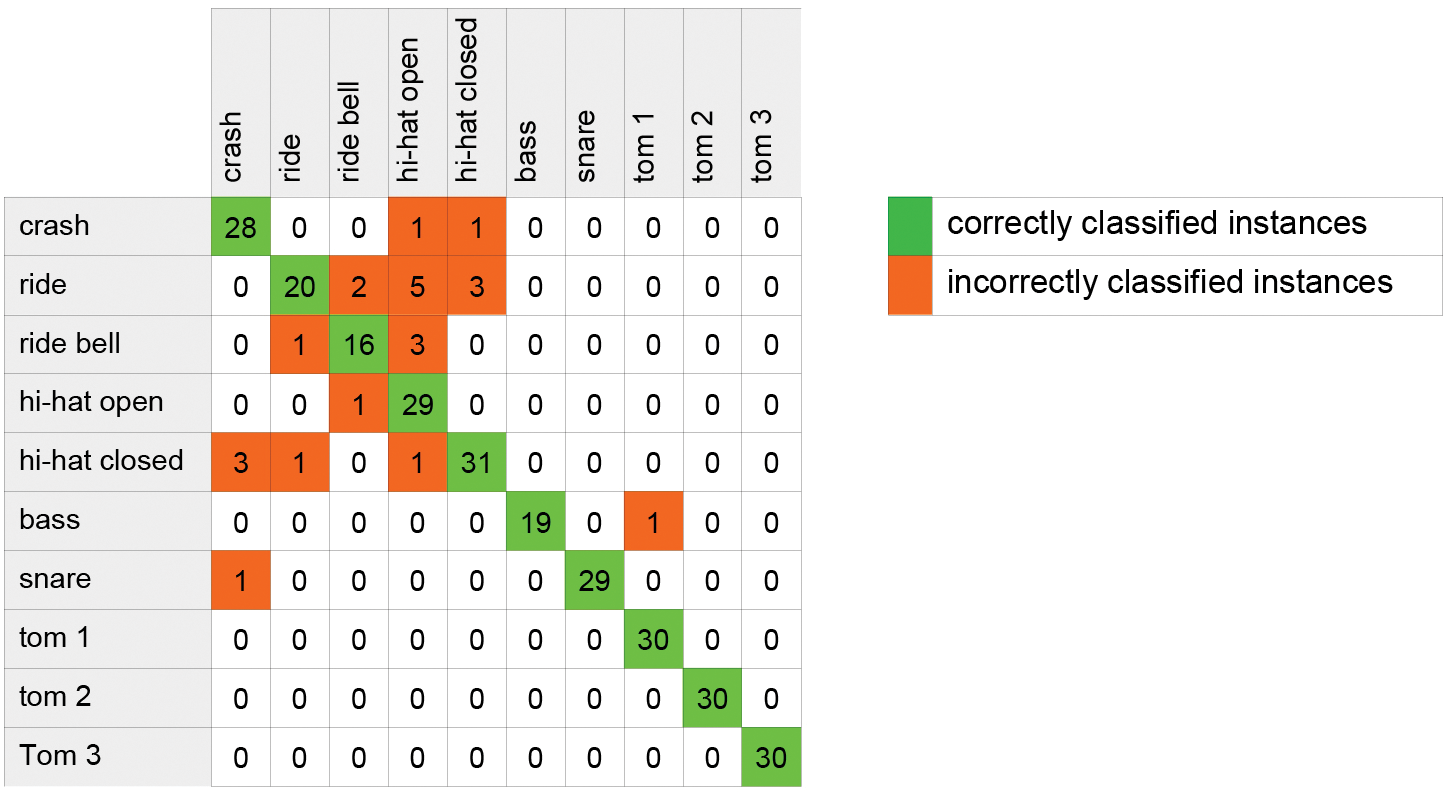
\includegraphics[width=.65\textwidth]{images/weka/weka_matrix_3.png}
	\caption{Confusion Matrix for J48 tree on feature set 3.}
	\label{fig:wekaMatrix3}
\end{figure}

\subsection{Classification by Templates Based on the Spectral Shape}
\label{section:method2}

The second method is based on the comparison of the spectral shape of the different stroke types. Therefore, in the training phase, templates for each trained drum and cymbal are created. These templates are used for comparison when classifying a stroke.

%a)create mean spectrum and use correlation coefficient for spectral shape comparison
%Dann brauchen wir ein Maß, das angibt, ob das Spektrum A und B
%übereinstimmt, wobei die Gesamtstärke keine Rolle spielen soll, nur die
%Form (spectral shape).  Dafür schlage ich vor:
%
  %sum (A .* B) / sqrt (sum (A.^2) * sum (B.^2)).
%
%Das ist aus der Statistik bekannt als (nicht zentraler)
%"Korrelationskoeffizient". Er ist 1, wenn A und B die gleiche Form
%haben, sonst kleiner und minimal -1.

%Sometimes, the exact relationship is not of interest, only the degree of association between two variables.
%This relationship (=association) is called the correlation between x and y. The strength of the correlation and whether it is negative or positive is given by a single statistic, r, the CORRELATION COEFFICIENT (also known as the Pearson Product Moment Correlation Coefficient):
%It is the ratio of the COVARIATION between x and y (corrected for their respective means) to the total variation in both x and y (once again corrected for their respective means)
%Covariation means just what the term implies - when (x - x-bar) is large (in absolute terms) and negative, is (y - y-bar) also large and negative? When x - x-bar is small and positive, is y - y-bar also small and positive?
%If (x - x-bar) is positive, and (y - y-bar) is positive, then the resulting term is positive
%If(x - x-bar) is negative, and (y - y-bar) is negative, then the resulting term is positive
%If (x - x-bar) is positive, and (y - y-bar) is negative, then the resulting term is negative
%If (x - x-bar) is negative, and (y - y-bar) is positive, then the resulting term is negative
%So you can see, that if x and y always match signs, the numerator will turn out to be positive, If they don't match, the numerator will be negative.
%The denominator is always positive due to the squaring, so whether or not r is positive or negative depends on the degree of matching in the numerator.
%A negative r indicates an inverse relationship (as x gets large, y gets large)
%r = 0 indicates no relationship between x and y
%A negative r indicates an inverse relationship (as x gets large, y gets small)

%Der empirische Korrelationskoeffizient als Maßzahl für die Stärke eines linearen Zusammenhangs wird mittels einer Normierung der empirischen Kovarianz durch das Produkt der Standardabweichung berechnet

The first approach to the comparison of the spectral shape was to use a correlation coefficient to compare the test instance $T$ with the training data. Therefore, a mean frequency spectrum $M$ from all training records for one class label is calculated. After that, the correlation coefficient is calculated from the vectors $T$ and $M$. The correlation coefficient $r$ is calculated by:

\begin{equation}
\label{eq:correlationcoefficient}
	r = \frac{\sum_{i=1}^{n}{(T_i * M_i)}}{\sqrt{\sum_{i=1}^{n}{(T_i^2)}\sum_{i=1}^{n}{(M_i^2)}}}
\end{equation}

%To test the correlation coefficient with MatLab\textsuperscript{\textregistered}, the following code was used:
%\lstinline{ r = sum (T .* M) / sqrt (sum (T.^2) * sum (M.^2)).}

This formula calculates the linear correlation in the spectral shapes of the two vectors $T$ and $M$ as a value between -1 and +1. If $T$ and $M$ represent the same drum or cymbal, the calculation shall return a value near one. The smaller the returned value, the smaller the correlation, the smaller the probability that the two spectra represent the same class label. Further information on correlation coefficients can be found in \autocite{Hedderich:2012}. 

%The empiric correlation coefficient $r_{xy}$ is described in \autocite{Hedderich:2012} as a measurement for the degree of the linear correlation between the variables $x_i$ and $y_i$. Like shown in the following formula (\ref{eq:correlationcoefficient}), it is calculated by the empiric covariance ($S_{xy}$) divided by the product of the standard deviations of $x_i$ and $y_i$ ($S_{x}S_{y}$). 
%
%\begin{equation}
%\label{eq:correlationcoefficient}
	%r_{xy} = \frac{S_{xy}}{S_x S_y} = \frac{\sum_{i=1}^{n}{(x_i-\bar{x})(y_i-\bar{y})}}{\sqrt{\sum_{i=1}^{n}{(x_i-\bar{x})^2}\sum_{i=1}^{n}{(y_i-\bar{y})^2}}}
%\end{equation}
%
%This formula returns a value $r$ between -1 and +1. A positive $r$ indicates a relationship between $x$ and $y$, a positive $r$ an inverse relationship. If $r = 0$, there is no relationship between $x$ and $y$. 

The use of the correlation between $T$ and $M$ leads to a low hit-rate, especially because of the varying amplitudes in a cymbal stroke. Here, the spectral shape differs a lot from stroke to stroke and also in the development of a single stroke. Thus, the correlation coefficient can be very small despite two equal drums are compared. This problem leads to a new approach that does not compare the test instance with the mean of the training data, but rather examines if the frequency bins of the test instance are located within an acceptable range. As displayed in figure \ref{fig:templates1}, this range is defined by two templates containing vectors. One defines the minimum and one the maximum limit for each bin in the drum strokes frequency spectrum. With this method a hit-rate of 97.2 \% is reached.

\begin{figure}[htb]
	\centering
	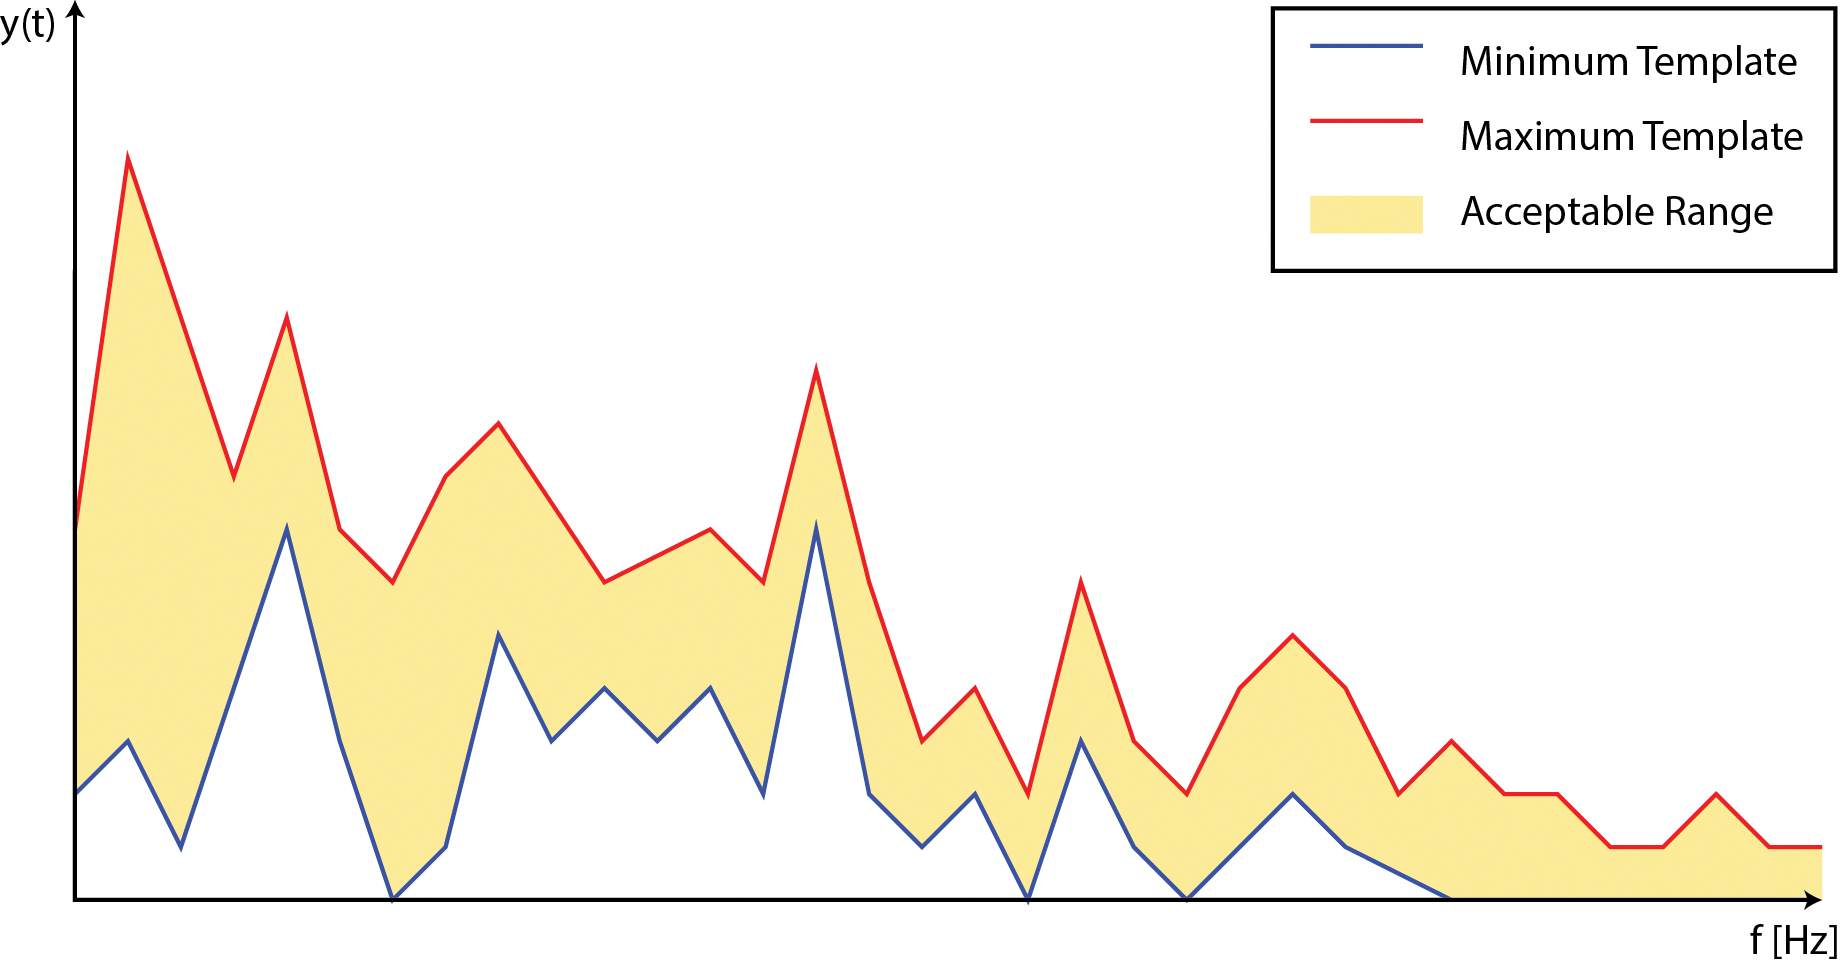
\includegraphics[height=6cm]{images/acceptable_range.png}
	\caption{Minimum and maximum template.}
	\label{fig:templates1}
\end{figure}

%If the resulting spectra of minimum and maximum amplitudes for a drum type are displayed, it can be seen, that the distance between the minimum and maximum bin at the most main peak positions is much smaller than the distance at non peak positioned bins. This leads to a smaller acceptable range in the classification step. The phenomena can be seen in figure \ref{fig:minmax}. It can be attributed to the fact that the main peaks of a stroke are more stable than other appearing frequencies, like shown in section \ref{section:classificationSpectrumAnalysis}. Because the main peaks can vary strong from stroke to stroke, the smaller acceptable range could cause errors in the classification step. This leads to the idea to create an additional template which only considers the peak positions within the frequency spectra of a record.

The creation of the templates is described in the following section. After that, three different methods for classification are tested. The methods are explained in sections \ref{section:shapeComparisonClassification1}, \ref{section:shapeComparisonClassification2} and \ref{section:shapeComparisonClassification3}.


\subsubsection{Template Creation} \label{section:shapeComparisonTemplates}

For the template creation the training data recorded as described in section \ref{section:training} is used. There are 24 different frequency spectra saved for each drum type. To use this frequency spectra for templating, each data record is pre-processed by onset detection, Fourier transform, noise reduction and normalization. Onset detection and Fourier transform are performed identically to the first classification method, which is described in section \ref{section:method1pre-processing}. For noise reduction and normalization an improved approach is used.

The new method for the noise reduction is developed in consideration of the usage in the final system. A future user might use a noisy microphone that interferes the drum sound, so it must be possible to filter every kind of noise. To realize that, an additional audio sequence containing silence is recorded. Thus, only the noise that is produced by the microphone is recorded. A frequency spectrum $N$ of the noise file is prepared for noise reduction as follows:

\begin{enumerate}
  \item The audio sequence $Y$ of the recorded file is loaded.
  \item The mean $M$ of three subsequent frames $Y_1, Y_2, Y_3$ extracted from the audio sequence is calculated, beginning with the first sample of the audio wave. Thereby, the frame size is 2048 samples, equal to the frame size used for the training set in section \ref{section:training}. The mean M is calculated by $(Y_1+Y_2+Y_3)/3$.
  \item The calculated mean $M$ is Fourier transformed to its frequency spectrum $N$ by MatLab\textsuperscript{\textregistered}s build in FFT function.
	\item The values of each amplitude bin $n_i$ in the frequency spectrum $N$ are transformed to its absolute values.
\end{enumerate}

%code
%[y_noise,fs] = audioread('silence.wav');
%noise = abs(fft(windowFunction.*((y(1:2048)+y(2049:4096)+y(4097:6144))./3)));

The calculated noise spectrum is subtracted from the absolute values of each training spectrum after multiplying it with a factor of 1.5. This way every frequency peak created by the noise is removed. Thus, only the frequency peaks produced by the appropriate drum persist. The factor 1.5 is chosen to ensure that the noise is also removed if there is a higher noise than in the recorded silence file. The noise reduction with this factor also produces some frequency bins with a negative value. Thus, after the subtraction, every bin with a value less than zero is set back to zero. After the noise is subtracted from the spectrum, the spectrum is normalized by dividing each amplitude value with the mean amplitude of all frequency bins. Thereby, it is important to do the normalization after the noise reduction because the noise peaks would adulterate the mean amplitude value and thus falsify the result. The normalization is needed because of the different amplitudes, which are created with every different stroke. They appear for instance in different powered strokes or different distances of the drums and cymbals from the microphone. As the frequency spectrum is inverted with respect to its center, only half the spectrum needs to be considered. Thus, only the bins 1 to 1024 are saved for further steps.

The entire pre-processing of each training records absolute frequency spectrum $A$ is performed as follows:

\begin{enumerate}
	\item Each value in the noise frequency spectrum $N$ is multiplied with a factor of 1.5.
	\item The noise frequency spectrum $N$ is subtracted from the frequency spectrum $A$.
	\item Each value in the frequency spectrum $A$ that is less than zero is set to zero.
	\item The mean amplitude $m$ of the frequency bins $a_i$ in the frequency spectrum $A$ is calculated.
	\item Each frequency bin $a_i$ in the frequency spectrum $A$ is divided by the mean amplitude $m$.
	\item The vector $A$ is shortened to half its size
\end{enumerate}

An example for the pre-processing of a drum stroke recording in MatLab\textsuperscript{\textregistered} is shown in listing \ref{lst:pre-processing2}.

\begin{lstlisting}[caption={pre-processing of an example drum stroke recording.},label={lst:pre-processing2}]
%read in audio files
[y,fs] = audioread('example.wav');
[y_noise,fs] = audioread('silence.wav');

%calculation of noise
noise = abs(fft(windowFunction.*((y_noise(1:2048)+y_noise(2049:4096)+y_noise(4097:6144))./3)));

%onset detection
onsets = detectOnsets(y);
onset = onsets(1);

%noise reduction
F=abs(fft(windowFunction.*y(start:start+windowSize-1)));
F=F-noise.*1.5;
F(F<0) = 0;

%normalization
F=F./mean(F);

%shorten frequency band
F=F(1:length(F)/2);
\end{lstlisting}

%code
%prepare training data
% noise reduction (add to training)
%Atmp=abs(fft(hamming(windowSize).*frame));
%Atmp=Atmp-noise.*1.5;
%Atmp(Atmp<0) = 0;
% normalization
%  Atmp=Atmp./mean(Atmp);
% returns frequency spectra of frames

After the training data is pre-processed, two different templates for each trained class label are created. Thereby, each recorded drum and cymbal is assigned to a class label. The different stroke types are also considered as separated classes.

%create template
%b)entire spectral shape with min max template
%returns AMin, AMax
%for every testframe of a drum:
%AMax = quantile(A, 0.99), AMin = quantile(A, 0.01);

The two templates are bordering an acceptable range for each frequency bin of a class. One of the two templates sets the maximum and one the minimum amplitude limits. Thus, each template is a vector of absolute frequency bins. These limiting values are $\alpha$-quantiles calculated by the appropriate frequency bins of all test records of the same class label. The use of the $\alpha$-quantiles avoids the use of outliers in the templates.

An $\alpha$-quantile is the smallest value in a set of increasing values which isn't exceeded by $\alpha$ percentage of all values. Thus, it is a threshold that divides a set of values in values smaller and values greater than the quantile. For example, the 60-quantile defines the value, where 60 \% of the values in the set are smaller and 40 \% greater, when compared. A detailed explanation can be found in \autocite{Hedderich:2012}. To calculate the $\alpha$-quantiles, the quantile function of MatLab\textsuperscript{\textregistered} is used. To this function, the value for $\alpha$ needs to be passed. For the created template, a 0.99-quantile is chosen for the maximum values and a 0.01-quantile for the minimum values. The template creation process is displayed in figure \ref{fig:templates1}.

%The book gives the following formula to calculate an \alpha-quantile:
%
%\begin{align}
	%x_{\alpha}=
  %\begin{cases}
		%\ \qquad \qquad x_{(k)}&: k=\lceil n*\alpha\rceil \qquad
		%\text{if $n*\alpha$ is not whole-number}\\
		%\frac12{x_{(k)}+x_{(k+1)}}&: k=n*\alpha \qquad \quad
		%\text{else}
  %\end{cases}
%\end{align}

%Ein Quantil ist ein Lagemaß in der Statistik. Anschaulich ist ein Quantil ein Schwellwert: ein bestimmter Anteil der Werte ist kleiner als das Quantil, der Rest ist größer. Das 25%-Quantil beispielsweise ist der Wert, für den gilt, dass 25% aller Werte kleiner sind als dieser Wert. Quantile erlauben ganz praktische Aussagen im Stile von „25% aller Frauen sind kleiner als 1,62 m“ – wobei 1,62 m hier das 25%-Quantil ist.
%Genauer ist das p-Quantil, wobei p eine reelle Zahl zwischen 0 und 1 ist, ein Wert einer Variablen oder Zufallsvariablen, der die Menge aller Merkmalswerte (salopp „die Verteilung“) in zwei Abschnitte unterteilt: Links vom p-Quantil liegt der Anteil p \equiv p \cdot 100\, \% aller Beobachtungswerte oder der Gesamtzahl der Zufallswerte oder der Fläche unter der Verteilungskurve; rechts davon liegt der jeweilige restliche Anteil 1-p \equiv (1-p) \cdot 100\, \%. Die Zahl p heißt auch der Unterschreitungsanteil.

%\begin{figure}[htb]
	%\centering
	%\includegraphics[height=2cm]{images/templates1.jpg}
	%\caption{Creation of templates for a minimum and maximum amplitude limit.}
	%\label{fig:templates1}
%\end{figure}

%Further there is a template which contains the mean values for each bin. It is created in the same way as the minimum/maximum templates, the only difference being that the mean value is calculated instead of using the quantile function.
%
%
%%c)only peaks
%%returns peaks
%%for every testframe of a drum:
%%[pks,locsPeaks] = findpeaks(Atmp(j,:), 'MinPeakHeight', max(Atmp(j,:))/peakThresholdDenom);
%The last template shows the distribution of peaks for the different trained drums. To build this template, there is created a vector $P_n$ with the same length as the training frequency spectra (2048 bins), for each class label. In this vector the amount of peaks over all training data records for the corresponding class label at each bin position is saved. The vectors $P_(1..n)$ are saved in a $mxn$ matrix, where the dimension m represents the frequency bin positions and n the different class labels. A vector $P_n$ is built as follows:
%
%\begin{enumerate}
	%\item for each training record A of a class label
	%\begin{enumerate}
		%\item The peaks in training record $A_i$ are extracted with MatLab\textsuperscript{\textregistered}s build in findpeaks function. This function returns the amplitudes $a$ and the positions $p$ of each peak within $A_i$.
		%\item At every position $p_j$ in the vector $P_n$, the existing value is increased by one.
	%\end{enumerate}
%\end{enumerate}
%
%The result of this procedure is a vector which shows the distribution of peaks within the test records for the considered class label. The more often a peak at a frequency bin position appears for a record of the considered class label, the higher is the value in the vector $P_i$ at this position. If there is no peak in any of the test records, the value is zero.
%
%The amplitudes $a_j$ are not used for templating because, especially for the cymbals, the peak amplitudes can vary strongly between different strokes, like examined in section \ref{section:classificationSpectrumAnalysis}. 
%
%The peak positions template creation is displayed in figure \ref{fig:templates2}.
%
%\begin{figure}[htb]
	%\centering
	%\includegraphics[height=2cm]{images/templates2.jpg}
	%\label{}
	%\caption{Creation of peak position template.}
	%\label{fig:templates2}
%\end{figure}


The MatLab\textsuperscript{\textregistered} code for the template creation is shown in listing \ref{lst:templates}. The parameter A is a matrix of all test records frequency spectra. The parameter n is the number of records for each class label. It is needed to separate the array A into matrices that contain only records of one class label type.

%code
\begin{lstlisting}[caption={Template creation},label={lst:templates}]
function[AMin,AMax]=createTemplates(A,n)
	AMin=zeros(length(A(:,1))/n,length(A(1,:)));
	AMax=zeros(length(A(:,1))/n,length(A(1,:)));
	locDrum=0;
	for i=1:n:length(A(:,1))				
		Atmp=A(i:i+n-1,:);
		locDrum=locDrum+1;				
		%% quantile
		AMax(locDrum,:)=quantile(Atmp,0.99);
		AMin(locDrum,:)=quantile(Atmp,0.01);   
	end
end
\end{lstlisting}
%\begin{lstlisting}[caption={Template creation},label={lst:templates}]
%function[AMin,AMax,AMean,Peaks]=createTemplates(A,n)
	%AMin=zeros(length(A(:,1))/n,length(A(1,:)));
	%AMax=zeros(length(A(:,1))/n,length(A(1,:)));
	%AMean=zeros(length(A(:,1))/n,length(A(1,:)));
	%Peaks=zeros(length(A(:,1))/n,length(A(1,:)));
	%locDrum=0;
	%for i=1:n:length(A(:,1))				
		%Atmp=A(i:i+n-1,:);
		%locDrum=locDrum+1;				
		%%% quantile
		%AMax(locDrum,:)=quantile(Atmp,0.99);
		%AMin(locDrum,:)=quantile(Atmp,0.01);
		%%% mean
		%AMean(locDrum,:)=mean(Atmp);        
		%%% peaks 
		%for j=1:n
			%[pks,locsPeaks]=findpeaks(Atmp(j,:),'MinPeakHeight',max(Atmp(j,:))/5);
			%for k=1:length(locsPeaks)
				%Peaks(locDrum,locsPeaks(k))=Peaks(locDrum,locsPeaks(k))+1;                
			%end
		%end
	%end
%end
%\end{lstlisting}

After the templates are build, they are used to classify new data instances. Therefore, the new instance is compared with all training instances within the templates. On basis of this comparison a class label is assigned to the tested instance. 

For the classification three different methods are tested, which are described in the following sections.

\subsubsection{Counting Frequency Bins in the Acceptable Range}
\label{section:shapeComparisonClassification1}

The first approach is to count the number of frequency bins of the test instance $A$ that are not inside the acceptable range of the template instance compared. The test instance is classified as the drum with the smallest number of bins outside the acceptable range. The acceptable range is defined by the minimum template matrix $AMin$ and the maximum template matrix $AMax$. They were described in section \ref{section:shapeComparisonTemplates}. 

Before a test instance can be used for the classification it has to be pre-processed just like the training instances in section \ref{section:shapeComparisonTemplates}. After pre-processing, the classification results are calculated as follows:

\begin{enumerate}
	\item A vector $R$ is defined for which the length is equal to the number of class labels in $AMax$.
	\item For each training class label $i$ in $AMax$:
		\begin{enumerate}
			\item A variable $hits$ is defined with the value zero.
			\item For every bin $j$ in the vector $A$ the variable $hits$ is increased by one if the bin $j$ is outside the acceptable area.
			\item The value in $R_i$ is set to the value of variable $hits$.
		\end{enumerate}
	\item The position of the minimum value in vector $R$ is returned as result.
\end{enumerate}

The appropriate MatLab\textsuperscript{\textregistered} code can be taken from listing \ref{lst:testQuantileA}.

%get ACrit for each drum by
\begin{lstlisting}[caption={testQuantileA},label={lst:testQuantileA}]
function[idxR]=testQuantileA(A,AMax,AMin)
	Results = zeros(1,length(AMax(:,1)));    
  for i = 1:length(AMax(:,1))
		hits = 0;  
		for j=1:length(A)
			if (A(j)<AMin(i,j) || A(j)>AMax(i,j))  
				hits=hits+1;
			end
		end
		Results(i) = hits; 
	end
	[minR,idxR]=min(Results);
end
\end{lstlisting}

Ten different class labels containing 29 different stroke types are trained. For the tests ten strokes for each different class label are recorded. To analyze the results, a confusion matrix is built that shows which test instances are classified as which class. For the first test, the confusion matrix shown in figure \ref{fig:matrix1} is built.

%describe results of matrix 1
% gesamt 290
% hit 1 - 39
% hit 2 - 127 (43,8%)
% 1+ 2 = 166 (57,24 %)
% miss - 124

%cymbals  (150)
% hit 1 - 22
% hit 2 - 60
% 1+2 = 72 (48%)
% miss - 78
% regular strokes - 48/50 (96%)
% (ohne laute schläge und schläge auf bow)

%drums (140)
% hit 1 -17
% hit 2 - 67
% 1+2 = 84 (60%)
% regular strokes - 37/50 (74%)
% (ohne laute schläge und schläge auf bow)

\begin{figure}[htb]
	\centering
	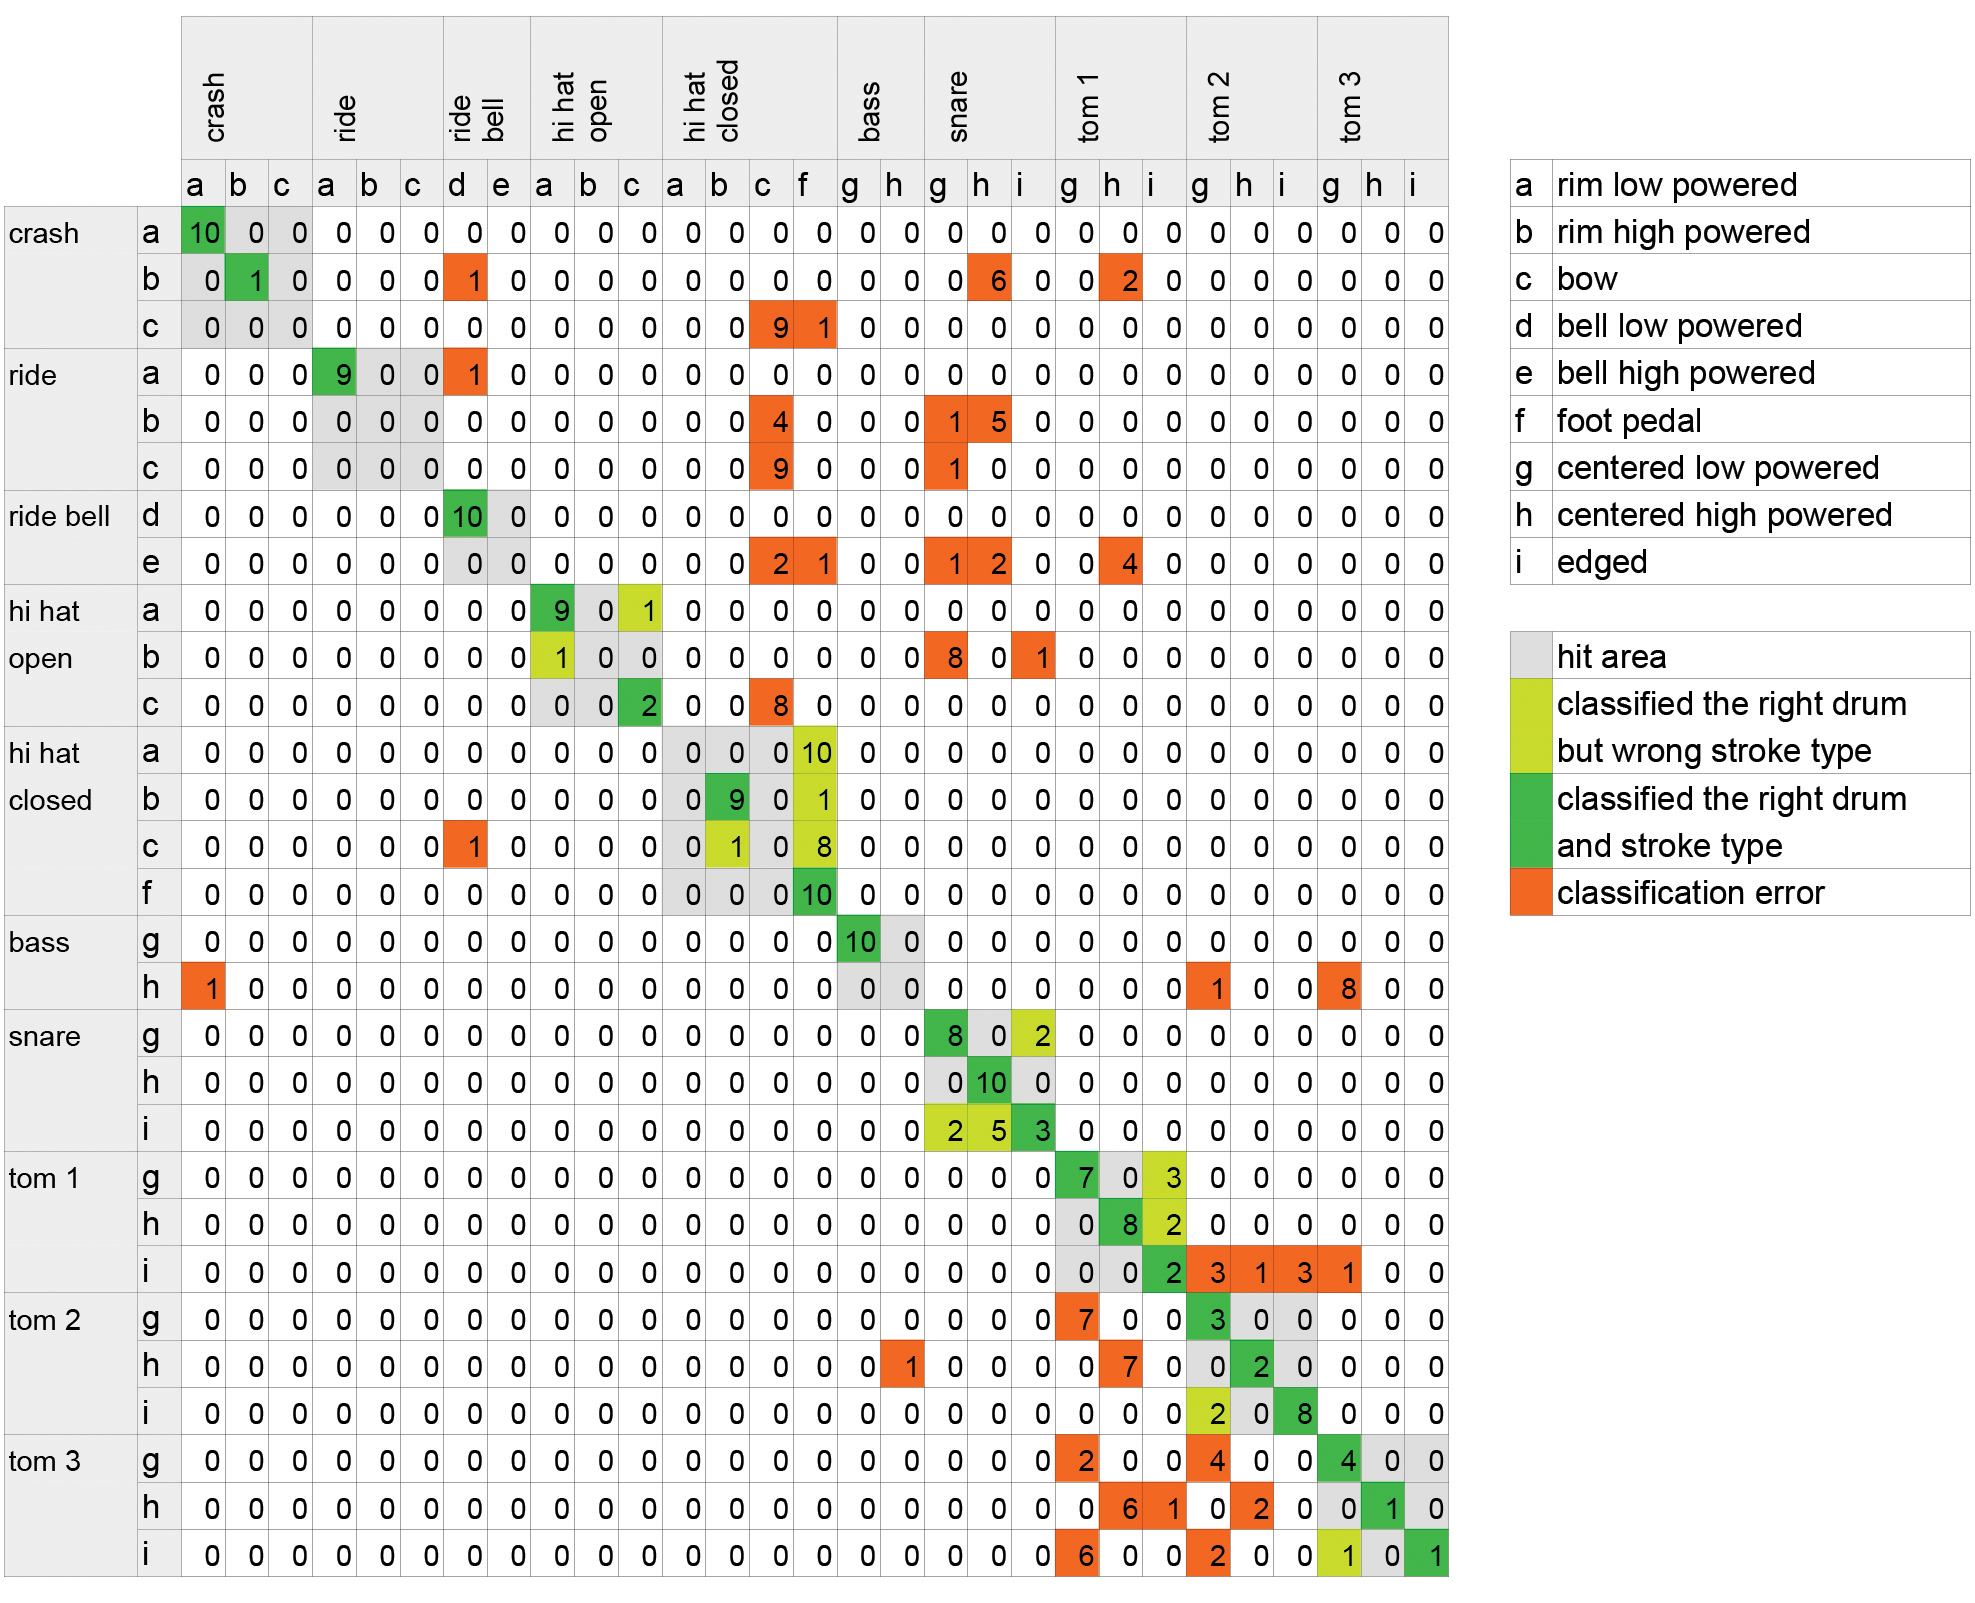
\includegraphics[width=\textwidth]{images/classification_matrix/matrix_test_1.png}
	\label{}
	\caption{Confusion matrix for counting frequency bins in the acceptable range.}
	\label{fig:matrix1}
\end{figure}

The confusion matrix in figure (figure \ref{fig:matrix1}) shows the  result of this test. A hit-rate of 57.2 \% is reached for correctly classified drums and cymbals. Furthermore, 43.8 \% of the stroke types are identified.

The hit-rate for cymbals only is 48.0 \%. Here appear classification problems, especially for loud strokes and strokes on the rim. If only regular strokes (low to medium powered strokes), which are the most used ones by drummers, are considered, the hit-rate reaches 96.0 \%. Further on, the closed hi-hat, which is usually the most frequently played cymbal, only shows one classification error out of 40 tests.

For drums only are achieved more correctly classified instances than for the cymbals. The hit-rate reaches 60.0 \% here. But if only regular powered strokes are considered, the hit-rate merely reaches 74.0 \%, whereas the cymbals were classified correctly by 96.0 \%.

% länge von A variieren
 %betrachten unterschiedlicher frequenzbänder
 %bestes Ergebnis mit Frequenzband ....

\subsubsection{Counting Frequency Bins in the Acceptable Range within a Predefined Frequency Band}
\label{section:shapeComparisonClassification2}

The second method for classifying drums and cymbals on basis of the minimum and maximum templates is developed by improving the preceding method.

Therefore, the distribution of frequency peaks in the frequency spectra of the different drums is considered. As described in section \ref{section:classificationSpectrumAnalysis}, the main peaks of the drums are located between 0 Hz and 2000 Hz, whereas the cymbals show peaks in all frequency ranges. This fact leads to errors when comparing the entire frequency spectra to classify a drum because drums cannot be differentiated above 2000 Hz. Furthermore, the frequency peaks of the cymbals are more stable in a lower frequency band.

Hence, especially to improve the hit-rate for the drums, the comparison of the frequency bins with the templates is reduced to a frequency band from 0 to 2000 Hz. In a window of 2048 frequency bins for the entire spectrum, 2000 Hz are equivalent to 93 frequency bins. The other parts of the classification algorithm as well as  the pre-processing remains constant to the first method, which was described in section \ref{section:method1}. 

The result of the developed method is displayed in the confusion matrix in figure \ref{fig:matrix2}. As expected, the hit-rate for the classification of the drums is clearly improved. 80.7 \% is reached now, whereas only 60.0 \% were reached in the last test now. This is a rise of 20.7 \%. For regular strokes on drums only the hit-rate is improved by 12.0 \% from 74.0 \% to 86.0 \%. The hit-rate for the cymbals could even be improved more than the hit-rate of the drums. It rises by 43.3 \% from 48.0 \% to 91.3 \%. If only the regular strokes on cymbals are considered, the hit-rate  of 96.0 \% is the same as in the last test. The over all hit-rate is improved by 29.3 \% in relation to the preceding test from 57.2 \% to a hit-rate of 86.5 \%. Thereby, the stroke type is classified correctly with 63.1 \%. This is an improvement of 19.3 \%.

\begin{figure}[htb]
	\centering
	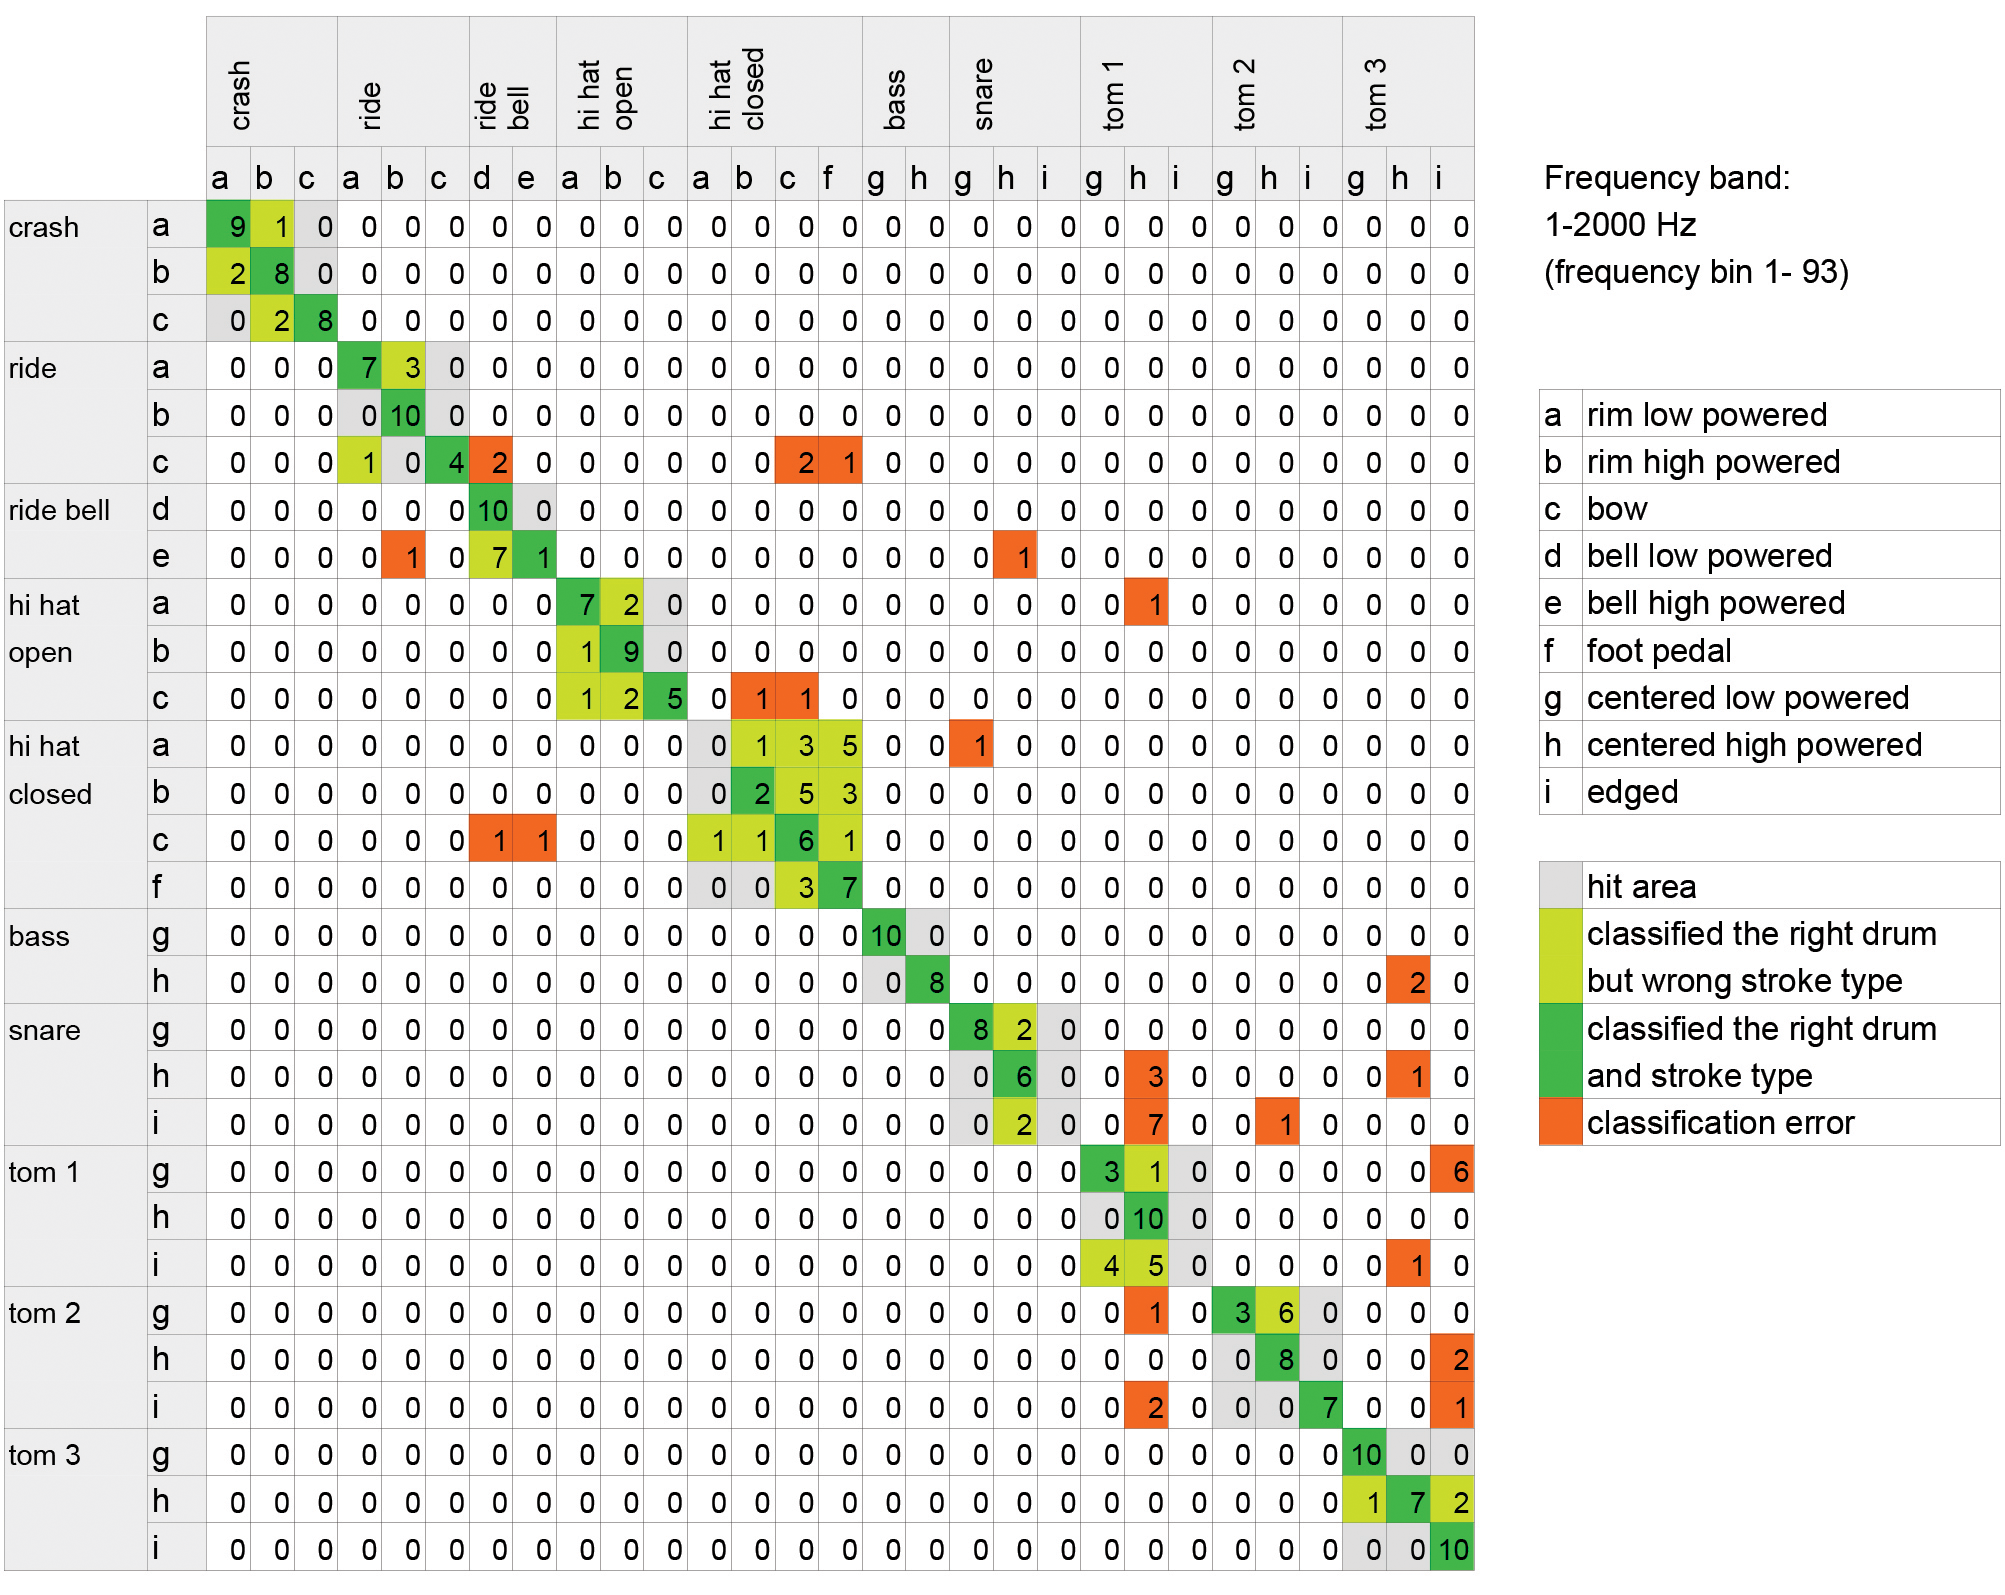
\includegraphics[width=\textwidth]{images/classification_matrix/matrix_test_2.png}
	\caption{Confusion matrix for counting frequency bins in the acceptable range within a predefined
frequency band.}
	\label{fig:matrix2}
\end{figure}

%describe results of matrix 2
% gesamt 290
% hit 1 - 68
% hit 2 - 183 (63.1%)
% 1+ 2 = 251 (86.5%)
% miss - 39

%cymbals  (150)
% hit 1 - 45
% hit 2 - 92
% 1+2 = 137 (91.3 %)
% miss - 13
% regular strokes - 48/50 (96%)
% (ohne laute schläge und schläge auf bow)

%drums (140)  
% hit 1 - 23
% hit 2 - 90
% 1+2 = 113 (80.7%)
% miss - 32
% regular strokes - 43/50 (86%)
% (ohne laute schläge und schläge auf bow)


\subsubsection{Calculating the Distance from the Acceptable Range}
\label{section:shapeComparisonClassification3}
%test quantile with distance from min/max

By the third classification approach, the developed algorithm is improved again. The method is based on the preceding approach, which was described in section \ref{section:shapeComparisonClassification2}. It focuses on the fact that there is only one stroke trained for each stroke type. This can cause errors in the preceding method because different strokes of the same stroke type can vary in their bin amplitudes. Thus, in some cases, the amplitude is not in the acceptable area, although the test stroke is compared with a matching template record. But in most cases the value is still close to the acceptable range. Usually, if the test record does not match the training record, the distance from the acceptable range is higher than the distance for non matching stroke types. Hence, the distance from the acceptable range is included in the algorithm. Instead of counting the bins outside the acceptable range as in the preceding approach, a simple distance function is applied. If a bin is placed outside the acceptable range, the distance of the bin to the area is added to the predefined distance variable \lstinline{distance}. The test instance is classified as the drum, where the template comparison returns the smallest distance value. The adapted MatLab\textsuperscript{\textregistered} code is shown in listing \ref{lst:testQuantileAD}.

\begin{lstlisting}[caption={testQuantileAD},label={lst:testQuantileAD}]
function[idxR]=testQuantileA(A,AMax,AMin)
	Results = zeros(1,length(AMax(:,1)));    
  for i = 1:length(AMax(:,1))
		distance = 0;  
		for j=1:372
			if A(j)<AMin(i,j)
				distance = distance + (AMin(i,j)-A(j));
      elseif A(j)>AMax(i,j)
				distance = distance + (A(j)-AMax(i,j));			
      end
		end
		Results(i) = distance; 
	end
	[minR,idxR]=min(Results);
end
\end{lstlisting}


For this approach, the best result is gained by considering a frequency band from 1 Hz to 8000 Hz. For a 2048 bin window this matches the bins 1 to 372. The error rate for the drums that appeared in the first method is reduced due to the distance. The frequency bins for drums in a frequency range over 2000 Hz are all near zero. Thus, the distance to the acceptable area is approaching zero, too.

The resulting confusion matrix is displayed in figure \ref{fig:matrix3}. For the 290 test instances, there are only eight classification errors. This is a hit-rate of 97.2 \%, whereas 70.3 \% of the instances are classified with the correct stroke type. If only regular strokes are considered this method reaches a hit-rate of 100 \%. 

Furthermore, all drums are classified with the right class label, 84.3 \% of them even with the correct stroke type. The class labels for cymbals are classified correctly with 94.6 \%, whereby for 57.3 \% of them the right stroke type is determined as well.


%describe results of matrix 3
% gesamt 290
% hit 1 - 78
% hit 2 - 204 (70.3%)
% 1+ 2 = 282 (97.2%)
% miss - 8

%cymbals  (150)
% hit 1 - 56
% hit 2 - 86 (57.3%)
% 1+2 = 142 (94.6 %)
% miss - 8
% regular strokes - 50/50 (100%)
% (ohne laute schläge und schläge auf bow)

%drums (140)
% hit 1 - 22
% hit 2 - 118 (84.3%)
% 1+2 = 140 (100%)
% miss - 0
% regular strokes - 50/50 (100%)
% (ohne laute schläge und schläge auf bow)


\begin{figure}[htb]
	\centering
	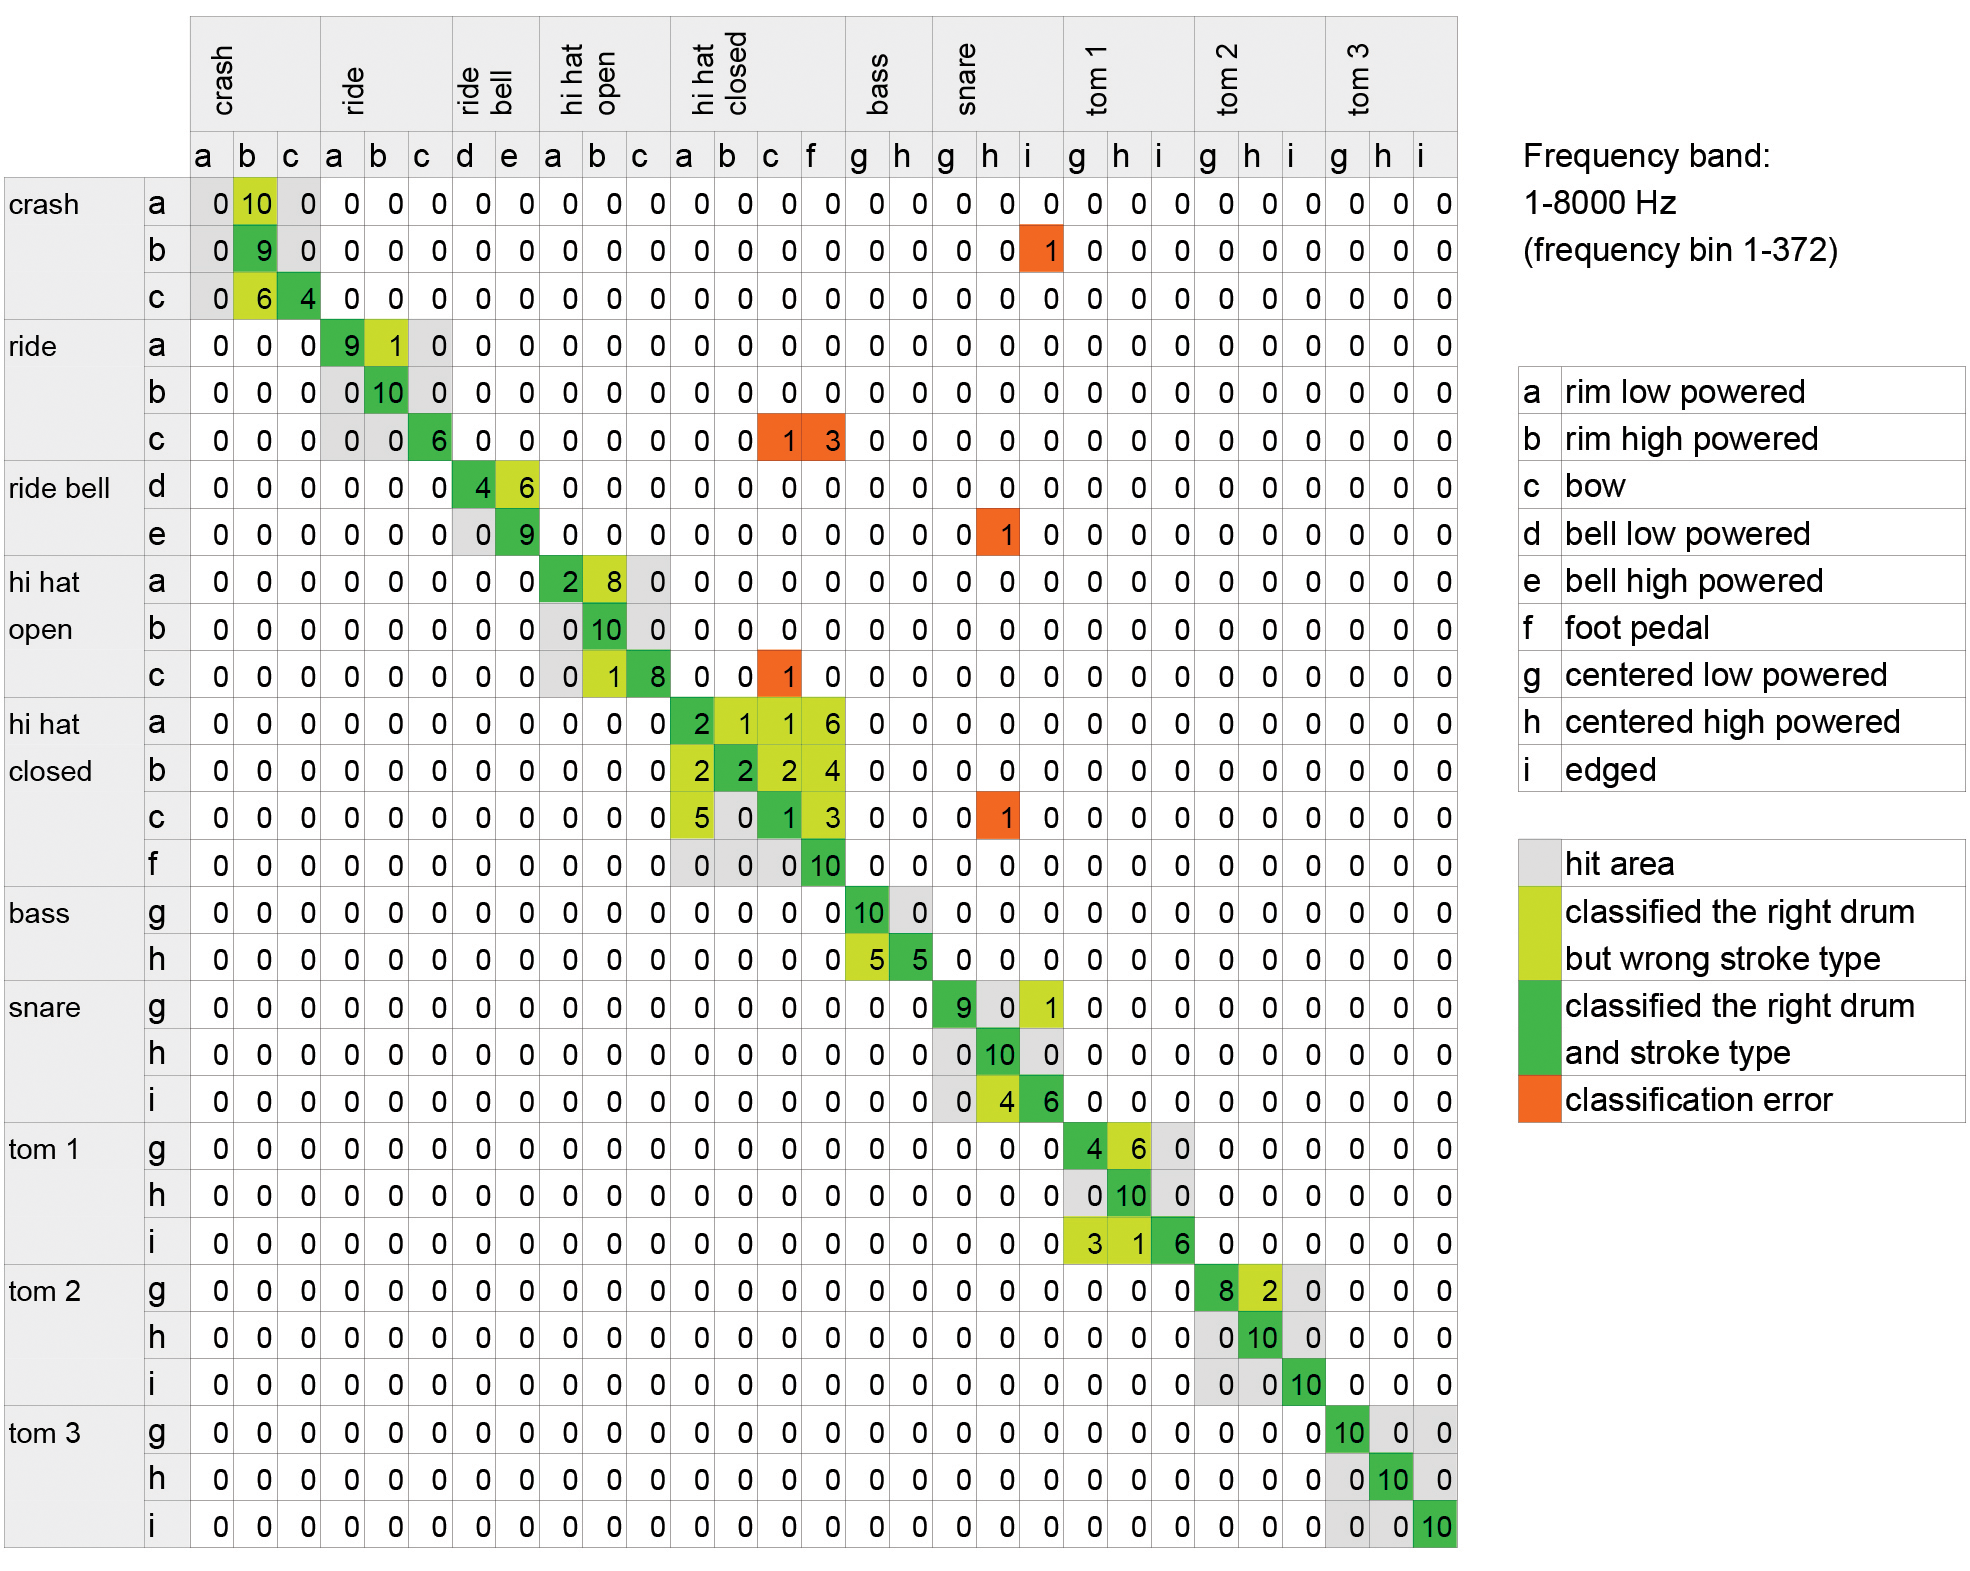
\includegraphics[width=\textwidth]{images/classification_matrix/matrix_test_3.png}
	\label{}
	\caption{Confusion matrix for calculating the distance from the acceptable range.}
	\label{fig:matrix3}
\end{figure}

%\newpage
%\subsubsection{The Use of Additional Features Using the Example Of the Steadiness}
%\label{section:shapeComparisonSteadiness}
%
%Next to the frequency spectrum, it is possible to use the approach described in the preceding with other features. An example feature which works with this approach is the steadiness, which was already used for the feature vector in the first classification method in section \ref{section:method1Features} of this thesis.

%test 4 quantile with distance from mean

%test 5 peaks

%Beim Testen passiert anschließend folgendes:
%Zunächst wird wieder ein Array mit 1024 Nullwerten erstellt und es werden die Peak Positionen des Testfiles gesucht.
%An jeder Position im Array, an der sich ein Peak befindet wird in der Trainingsmatrix der höchste Wert gesucht und im Array gespeichert. Dieser Wert repräsentiert die Drum, die am ehesten zu diesem Peak passt. 
%Nachdem alle Werte ins Array eingetragen sind werden diese gezählt. Der Wert, der am häufigsten vorkommt gewinnt. Als diese Drum wird das Testfile Klassifiziert.

%Result matrix:

%\subsubsection{Test results}



%%
	%\centering
	%\includegraphics[height=2cm]{images/templates12.jpg}
	%\label{}
	%\caption{Creation of templates for a minimum and maximum amplitude limit.}
	%\label{fig:templates12}
%\end{figure}]
